\documentclass[english,nohyper,titlepage]{tufte-handout}\usepackage[]{graphicx}\usepackage[]{color}
%% maxwidth is the original width if it is less than linewidth
%% otherwise use linewidth (to make sure the graphics do not exceed the margin)
\makeatletter
\def\maxwidth{ %
  \ifdim\Gin@nat@width>\linewidth
    \linewidth
  \else
    \Gin@nat@width
  \fi
}
\makeatother

\definecolor{fgcolor}{rgb}{0.345, 0.345, 0.345}
\newcommand{\hlnum}[1]{\textcolor[rgb]{0.686,0.059,0.569}{#1}}%
\newcommand{\hlstr}[1]{\textcolor[rgb]{0.192,0.494,0.8}{#1}}%
\newcommand{\hlcom}[1]{\textcolor[rgb]{0.678,0.584,0.686}{\textit{#1}}}%
\newcommand{\hlopt}[1]{\textcolor[rgb]{0,0,0}{#1}}%
\newcommand{\hlstd}[1]{\textcolor[rgb]{0.345,0.345,0.345}{#1}}%
\newcommand{\hlkwa}[1]{\textcolor[rgb]{0.161,0.373,0.58}{\textbf{#1}}}%
\newcommand{\hlkwb}[1]{\textcolor[rgb]{0.69,0.353,0.396}{#1}}%
\newcommand{\hlkwc}[1]{\textcolor[rgb]{0.333,0.667,0.333}{#1}}%
\newcommand{\hlkwd}[1]{\textcolor[rgb]{0.737,0.353,0.396}{\textbf{#1}}}%

\usepackage{framed}
\makeatletter
\newenvironment{kframe}{%
 \def\at@end@of@kframe{}%
 \ifinner\ifhmode%
  \def\at@end@of@kframe{\end{minipage}}%
  \begin{minipage}{\columnwidth}%
 \fi\fi%
 \def\FrameCommand##1{\hskip\@totalleftmargin \hskip-\fboxsep
 \colorbox{shadecolor}{##1}\hskip-\fboxsep
     % There is no \\@totalrightmargin, so:
     \hskip-\linewidth \hskip-\@totalleftmargin \hskip\columnwidth}%
 \MakeFramed {\advance\hsize-\width
   \@totalleftmargin\z@ \linewidth\hsize
   \@setminipage}}%
 {\par\unskip\endMakeFramed%
 \at@end@of@kframe}
\makeatother

\definecolor{shadecolor}{rgb}{.97, .97, .97}
\definecolor{messagecolor}{rgb}{0, 0, 0}
\definecolor{warningcolor}{rgb}{1, 0, 1}
\definecolor{errorcolor}{rgb}{1, 0, 0}
\newenvironment{knitrout}{}{} % an empty environment to be redefined in TeX

\usepackage{alltt}
\usepackage[unicode=true,pdfusetitle,bookmarks=true,bookmarksnumbered=false,bookmarksopen=false,
            breaklinks=false,pdfborder={0 0 0},backref=false,colorlinks=true]{hyperref}
%%% fonts            
%\usepackage{beramono}
% \renewcommand*\familydefault{\ttdefault} % in order to have bera as default
%\usepackage{helvet}
%\renewcommand*\familydefault{\sfdefault}  % helvetica
\usepackage{charter}
\usepackage{helvet}
\renewcommand{\familydefault}{\rmdefault}
\usepackage[latin9]{inputenc}

\usepackage{color}
\usepackage{natbib}
\usepackage[export]{adjustbox}
\usepackage{babel}
\usepackage{graphicx}

\usepackage{tabu} % for better tables

\usepackage{amsmath} % for alignment and various

% link color
\hypersetup{urlcolor= RoyalBlue, citecolor=RedOrange, linkcolor=RedOrange}

%%% title etc.
\title{\Huge R \& Social Science \\ \noindent \small Getting started with applied use of R in the Social Sciences}
\author{{\small Michael Clark\\
         \noindent Center for Social Research\\
         \noindent University of Notre Dame\\}}

%%% header
\fancyhf{}% clear previous contents of running heads/feet
\fancyhead[RE]{\footnotesize{CSR\qquad{} \thepage}}
\fancyhead[LO]{\footnotesize{\thepage \qquad{}R in the Social Sciences}}
%\rhead{Bayesian Basics}

%%% remove indent from tables
% \let\TAB\tabular
% \renewcommand\tabular{\noindent\TAB}    

\graphicspath{{Figures/}}
\IfFileExists{upquote.sty}{\usepackage{upquote}}{}
\begin{document}
\maketitle

\pagebreak

\tableofcontents

\pagebreak

%%%%%%%%%%%%%%%%%%%%%%%%%%%%%%%%%%%%%%
\part{Preface}
\marginnote{Current draft \today{}.}
\section{My Journey to R}


A little background.  While I could go into boring detail, suffice it to say, and as much as it pains me to do so, I was born an SPSS menu-clicker, as far as my stats training goes.  I started making the switch over 10 years ago thanks to an acquaintance who had spent more time in the stats world and was using R.  Unlike SPSS, whose base offering seemed to center around  the content of statistics textbooks of the 1970s, I found that R could easily pull off the modern methods statistically minded individuals in social science and psychology were requesting that applied researchers do.  But it could do a lot more, and the only limiting factor was me.  I never learned a thing about statistics using SPSS, while I was learning something new all the time with R. When I began using it to teach, and despite the students' having the very same grumblings I had about programming, there would actually be light bulbs coming on when they used it.  Again, this isn't something I witnessed with SPSS.  It was also nice to have a tool they and anyone could afford.  Due to R's rise in popularity you can now get a free student, i.e. crippled, version from SPSS, as well as use R code within it's syntax, as well as offering a developer pack so that you can use R to make SPSS better (for a price of course).  If nothing else, \emph{even SPSS's own founder jumped ship to R years ago}, saying "R is an absolutely massive advancement on the kind of analytics I invented. It's an opportunity to change the game in the fastest-growing field in software."\sidenote{I'm not sure what analytics he's referring to as having invented.}.  

R is both free and freeing.  It is not tied down to any particular discipline or industry persuasion.  It is easily modified, expanded, and enhanced.  In short, R is there to do with what you want statistically, and the possibilities are endless.  You will learn more about your data, your models, and about statistics, by programming in R than you would using canned routines in a typical statistics package. Is it perfect? No, no programming language is.  But it will do what you want, and what else really matters aside from that?

While personally I feel the writing was on the wall for applied researchers years ago, the following document will attempt to provide specific reasons for someone else to make a similar switch, particularly those in the social sciences.  By the way, this document was created \emph{with R} in the same environment used for statistical programming\sidenote{Using knitR and other packages, mixed with \LaTeX}.  For other examples you can see my documents here. 

\pagebreak{}


% !Rnw root = DDR.Rnw


\part{R on the Rise}
R's popularity has been meteoric over the past 10 or more years.  But you don't have to take my word for it.  As a starting point we can note a Google trends plot over the past 10 years.  Note that for the following, since there was no special topic for SPSS programming or statistics, or SAS outside of SAS Institute, so their absolute numbers may be inflated by other things (especially SAS), but the absolute values aren't as important for our purposes as the trends.  The only one notably on the rise is R.

\bigskip
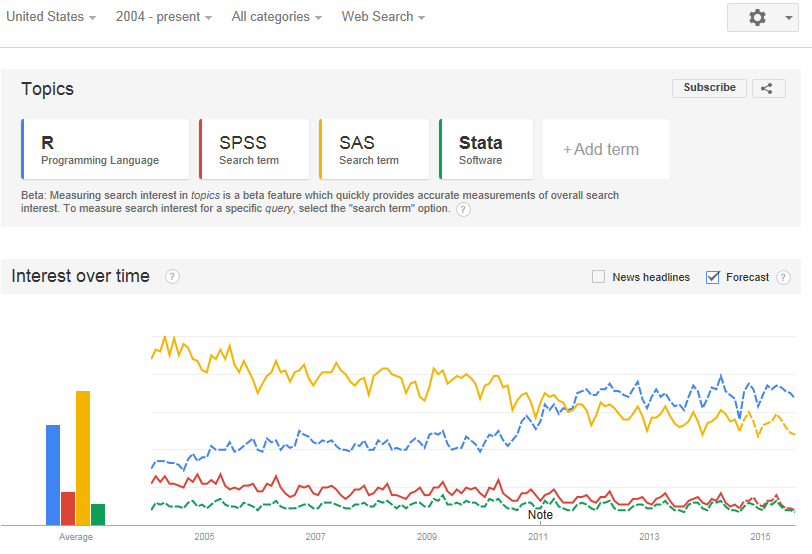
\includegraphics[scale=.35]{trendssmall}
\bigskip


\section{R Popularity Summarized}
In fact there is a regularly updated \href{http://r4stats.com/articles/popularity/}{website} devoted to the popularity of R, maintained by the author of books that help people to migrate from SAS, SPSS, and Stata\sidenote{I should note that I've never come across a book with a title that goes in the reverse direction.  If you are proficient at R, you have enough programming skill to learn the others, but there is also no need to.}.  I will provide a brief summary\sidenote{Several of these are based on results from two years ago.}.

\begin{description}
  \item[Job Advertisements] For analytics jobs, R is on the rise while SAS and SPSS are stagnate and other statistical packages aren't even common. You'd be better off with Python than SPSS skills in the modern analytics world.
  \item[Google Scholar] Not exactly telling as most articles seem to want you to think that their statistics arise magically from the authors' skulls and the tools used are left uncited, but SPSS has simply plummeted in Google scholar hits since 2005, while SAS has lost notable ground since 2008. R, and even  Stata, have gained.
  \item[Published Books]  R has provided SAS and SPSS a 20 year head start, but has already caught up to SPSS, while SAS is still a ways off.  
  \item[Website Popularity] R is second only to SPSS in terms of links to its homepage, though really that is a comparison to IBM as IBM.com is SPSS's homepage.  SAS is a distant second, and Stata notably lower than SAS.
  \item[Blogs]  It's not even remotely close here.  There are 550 blogs currently listed at R-Bloggers.com, while SciPy (Python library) has only a tenth devoted to it, which is still more than SAS and Stata combined.  
  \item[Discussion Lists] From their own to discussion forums to popular programming sites like CrossValidated, StackOverflow and TalkStats, R dominates. SAS catches up at places like LinkedIn and Quora.  SPSS and Stata are way off the pace.
  \item[Popularity Measures] Several (obviously limited) surveys at sites like KDNuggets ask big data and analytics folks what tools they're using, and R is again more widely used than traditional statistics packages, followed by SAS and SPSS.  Stata isn't even on the map here.  
\end{description}


\marginnote{R has really become the second language for people coming out of grad school now, and there's an amazing amount of code being written for it. You can look on the SAS message boards and see there is a proportional downturn in traffic. ~ Max Kuhn, associate director of nonclinical statistics at Pfizer in a New York Times article on R from \emph{2009}. }
There are plenty of bones to pick about trying to assess any of the above outside of a few of the measures, but I think it's safe to say that R is very popular right now.  Companies like Google, aside from general programmers, aren't looking for SPSS and SAS proficiency, they're hiring R programmers. For data driven graphics, the NY times graphics team is using R and other programming languages like JavaScript on the backend, not any other statistical packages\sidenote{See the blog of their Graphics Editor \href{http://chartsnthings.tumblr.com/post/22471358872/sketches-how-mariano-rivera-compares-to-baseballs}{here} and \href{http://chartsnthings.tumblr.com/post/49236510636/charting-skill-and-chance-in-the-n-f-l-draft}{here} for more insight into their process.}.   So if industry is shifting to R and other programming tools, and the statistical community long ago adopted R as their primary tool of choice, it stands to reason applied researchers might want to use it as well, and the fact is a great many of them already are.

In the following I'll show some specific R tools framed within social science applications.  Nowadays it's not uncommon to find someone doing social science research might be a physicist, biologist, or computer scientist, though I have more traditionally trained social scientists in mind.  I'll specifically note a few applications in political science, psychology and sociology.  After that I'll provide specific programming examples to show how easy it is relative to other programs.  Then I'll suggests some additional thoughts that go beyond the standard approaches.




% !Rnw root = DDR.Rnw



\part{Overview of R}
I'm not going to provide a full introduction to R.  If you want that you can see my introduction \href{http://www.nd.edu/~mclark19/learn/Introduction_to_R.pdf}{here}.  However an overview is in order to give one the proper context for comparison to alternatives.

\section{R is not a stats package}
R is not a "stats package".  R is a true \emph{programming language}\sidenote{Contrast with a syntax developed for using punch cards on mainframe computer.}- it is a dialect of S, which has won awards and has almost as long a history as SAS and SPSS.  Beyond that it is best thought of as a programming environment within which statistics is conducted.  In a sense it has more in common with Python than it does with the syntax used in stats packages, and that has far-reaching effects for data manipulation and exploration, post-processing of models, and visualization.

Base R has most of the functionality you'd find in a traditional statistics package and beyond, plus a system for creating fantastic visualizations.  R is open-source, which means that one can inspect and modify its contents freely.  Because of its programmability, it is easy for others to provide additional functionality in the form of \emph{packages}, to date of which there are almost 6000.  So with R you have a fully functioning statistical system to start with, and its open nature and programming language allow others to add more features all the time.  This is part of the reason for its popularity, as well as it always being able to provide cutting edge techniques to more applied users.

You will have to beef up some programming skills to use R effectively, but serious statistical analysis has always required that, at the very least for the initial data preparation.  Only now it will be easier.  R is what is referred to in programming languages as an \emph{object-oriented} programming, and once you get used to it for your statistical and data needs, it will be hard if not impossible to go back to the inefficient methods of statistical package syntax\sidenote{Some offer more developed programming languages now, e.g. Stata's Mata language, but the user communities are relatively smaller because those who program like that have long had other alternatives.}.  Yes you can use those to do many of the same commonly employed approaches to data manipulation, and it is easy to get basic model results. However with R it is no more difficult to work with 1 vs 10 or 100 data sets, you don't have to create explicit representations of variables to use them in modeling or for simple data exploration, you can avoid loops entirely for common iterative tasks, prediction is built in to the vast majority of modeling functions, you have many plotting methods for results of analyses built-in, you can easily call in or even write and use other languages for certain tasks, and you can easily write your own functions (even implicitly) and modify others, engage in interactive graphics, write dynamic, publish-ready documents. etc.  One key idea to note- \emph{you do not have to be a great R programmer to use it effectively and do some pretty amazing things, but you do have to be an excellent programmer to do those things in other statistics packages}.

Much of the apprehension I see from non-R users is that because of the handcuffing of their own tools, they simply cannot imagine the sorts of things they \emph{could} be doing with R.  As I started using it, my initial attempts would make me wonder if I could take it further.  Once I did, I could imagine what else I could do, and tried that. And this cycle continues to this day. As mentioned, the only limitation to what you can do with R is you.

The later demonstrations will hopefully provide greater insight on the R approach in the social sciences.  For now it is simply important to note that R is fundamentally different from traditional statistics packages.  It will take some getting used to, but the payoff is worth it, and you wouldn't be doing research in the first place if you were afraid of hard work.




% !Rnw root = DDR.Rnw



\part{R for Political Science}
A lot of political scientists seem to like Stata, and for good reason, it's simply a good statistical tool.  But what might R offer to a political scientist?  The answer is plenty.

As a starting point Much of political science methodology is based on econometrics, and there is a \href{http://cran.r-project.org/web/views/Econometrics.html}{slew} of packages that would fall within that \href{http://cran.r-project.org/web/views/SocialSciences.html}{realm}.  There are political scientists who have provided specific packages such as \href{http://datascience.iq.harvard.edu/zelig}{Gary King and the IQSS group at Harvard}, the \href{http://pscl.stanford.edu/}{Political Science Computational Lab} at Stanford, and even from the \href{http://mcmcpack.berkeley.edu/}{President of the Society for Political Methodology}.  On the data side one can use a packages such as \href{http://cran.r-project.org/web/packages/WDI/index.html}{WDI} for world bank data, \href{http://cran.r-project.org/web/packages/dvn/index.html}{dvn} for access to the Dataverse Network, and a more recent offering, \href{http://cran.r-project.org/web/packages/psData/index.html}psData, that also looks 

\section{Example}
Let's provide a political science demonstration.  Recently I was interested in looking at investigating cliques within the congress, and as a starting point we can examine how they vote on bills and where they line up within their party.  Let's say I would like rollcall data from the current House of Representatives and make map that reflects their spatial position in terms \emph{ideal point estimation}.  This is not the place for details but instead merely a place to show how easy it can be to go from something to nothing.

Getting the data from voteview.com and estimating a quick model is easy enough with the \emph{\textcolor{blue}{pscl}} package, which has specific functionality to create a rollcall class object ready for analysis, and the function to do analysis based on MCMC.  I'll choose the last completed legislature, and stick to defaults for ease of presentation.  The default plot is to the right.

\marginnote{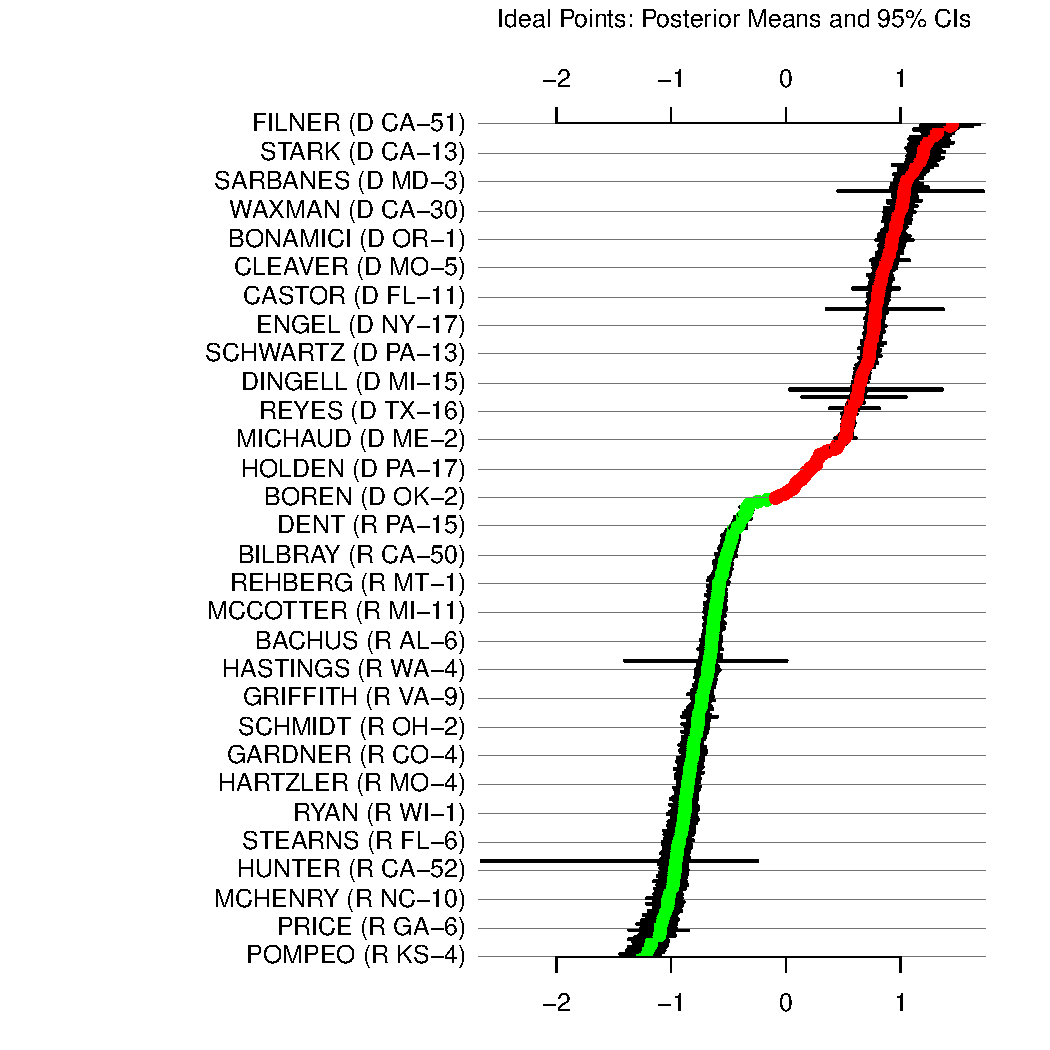
\includegraphics[scale=.25]{idealModel}}
\begin{knitrout}\footnotesize
\definecolor{shadecolor}{rgb}{0.969, 0.969, 0.969}\color{fgcolor}\begin{kframe}
\begin{alltt}
\hlkwd{library}\hlstd{(pscl)}
\hlstd{rc112} \hlkwb{=} \hlkwd{readKH}\hlstd{(}\hlstr{'ftp://voteview.com/hou112kh.ord'}\hlstd{,}
               \hlkwc{desc}\hlstd{=}\hlstr{'112th U.S. House of Representatives'}\hlstd{)}
\hlstd{idealModel} \hlkwb{=} \hlkwd{ideal}\hlstd{(rc112)}
\hlkwd{plot}\hlstd{(idealModel)}
\end{alltt}
\end{kframe}
\end{knitrout}

The idealModel object has the estimated values for each member of the House.  Now we can create a map that reflects them in geographic space as well.  I downloaded the shapefile from the \href{http://cdmaps.polisci.ucla.edu/}{UCLA political science department}, but know that there is plenty of mapping functionality already available for state, county and even census tract/block level mapping in R. 
\marginnote{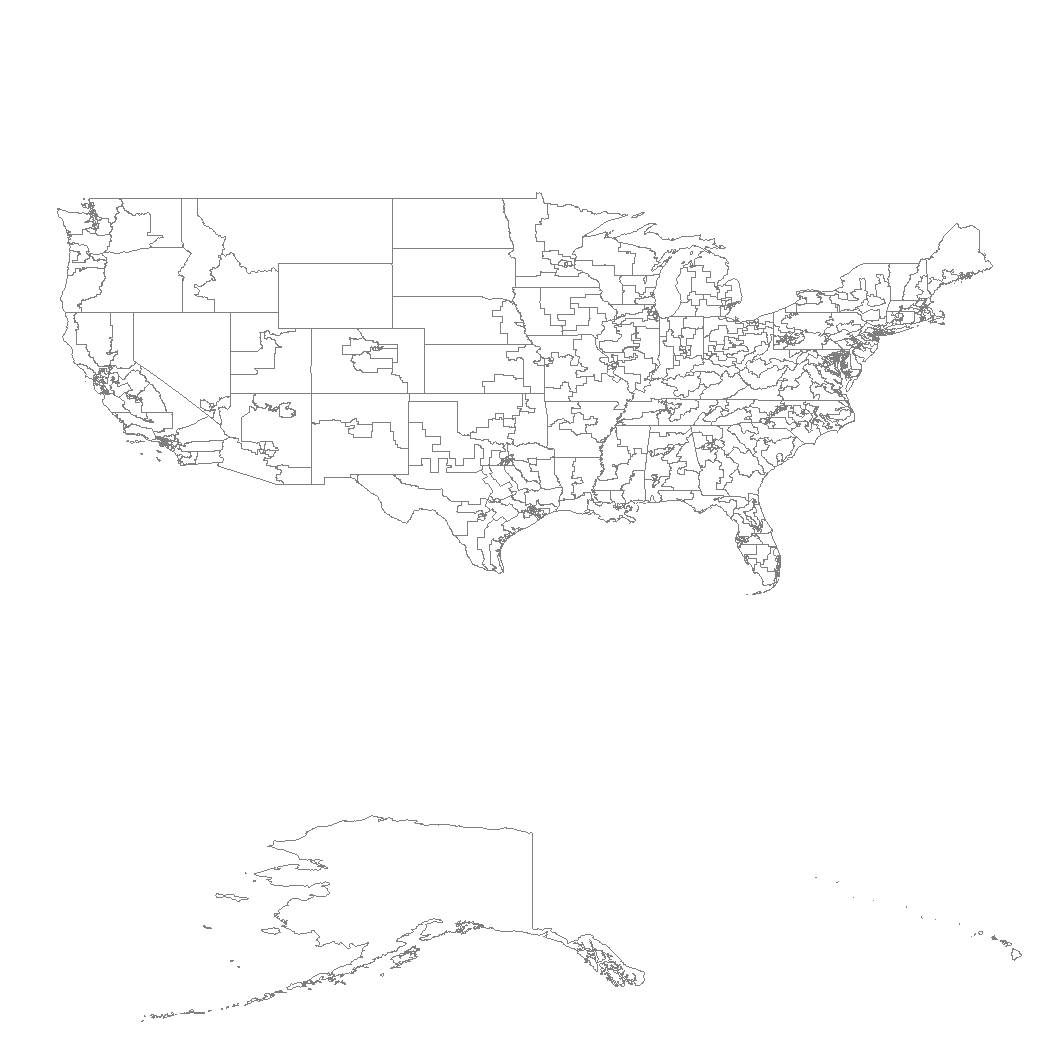
\includegraphics[scale=.25]{initialDistMap}}

\begin{knitrout}\footnotesize
\definecolor{shadecolor}{rgb}{0.969, 0.969, 0.969}\color{fgcolor}\begin{kframe}
\begin{alltt}
\hlkwd{library}\hlstd{(maptools)}
\hlstd{congressDist} \hlkwb{=} \hlkwd{readShapePoly}\hlstd{(}\hlstr{'PolySci/districtShapes112/districts112.shp'}\hlstd{)}
\hlkwd{plot}\hlstd{(congressDist)}
\hlnum{NA}
\end{alltt}
\end{kframe}
\end{knitrout}

\begin{knitrout}\footnotesize
\definecolor{shadecolor}{rgb}{0.969, 0.969, 0.969}\color{fgcolor}\begin{kframe}
\begin{verbatim}
## pdf 
##   2
\end{verbatim}
\end{kframe}
\end{knitrout}

Trying to transfer data values onto maps is rarely a straightforward process.  While there are a several issues to contend with, we'll note one particular example I came across.  Within both the map object \texttt{congressDist} and the ideal object \texttt{rc112} I created above resides a data set with district codes.  These match for the most part but we need to create a unique identifier so that, e.g. the first district in each state goes to the correct state.  This can be easily accomplished by creating a new unique identifier that just combines state and district.  Unfortunately the data associated with the map has long form state names, while the roll call data uses abbreviations, so we'll need to find a way around this.

Turns out R has state long form names and abbreviations in its base installation in the objects called \texttt{state.abb} and \texttt{state.name}, and changing from one form to the other in our own data set then becomes easy.  After extracting the rollcall data.frame (\texttt{rcdat}), we can more easily play with it directly, then merge it into the map's data set.

The final map I show drops Alaska and Hawaii for easier inspection. Colors fade to white as they get closer to overall mean of the legislators.  I also add a comparison of party identification for comparison.  One can see, for example, that Democratic representatives (blue) in otherwise Republican states (e.g. in Oklahoma and Arkansas) and regions appear to be drawn more away from their typical party line.


%\marginnote{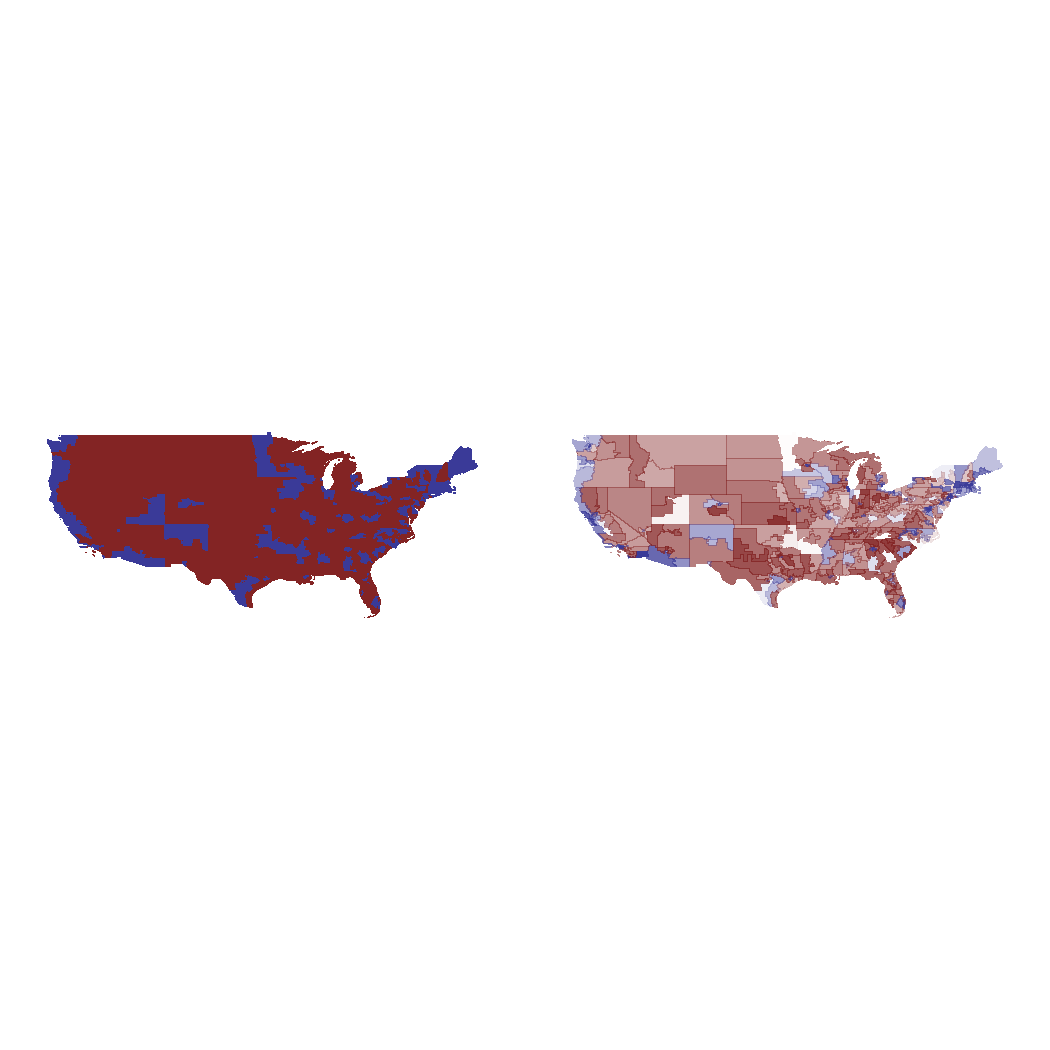
\includegraphics[scale=.25]{idealMap}}


\begin{knitrout}\footnotesize
\definecolor{shadecolor}{rgb}{0.969, 0.969, 0.969}\color{fgcolor}\begin{kframe}
\begin{alltt}
\hlcom{# create a new identifier that combines the state with the }
\hlstd{rcdat}\hlopt{$}\hlstd{cd2} \hlkwb{=} \hlkwd{paste0}\hlstd{(rcdat}\hlopt{$}\hlstd{state, rcdat}\hlopt{$}\hlstd{cd)}

\hlcom{# do the same for the map data, simultaneously converting the full name to }
\hlcom{# postal abbreviation}
\hlstd{congressDist}\hlopt{@}\hlkwc{data}\hlopt{$}\hlstd{cd2} \hlkwb{=} \hlkwd{paste0}\hlstd{(state.abb[}\hlkwd{match}\hlstd{(congressDist}\hlopt{@}\hlkwc{data}\hlopt{$}\hlstd{STATENAME, state.name)],}
                               \hlstd{congressDist}\hlopt{@}\hlkwc{data}\hlopt{$}\hlstd{DISTRICT)}

\hlcom{# examine and see that they have the same form}
\end{alltt}
\begin{verbatim}
##      [,1]  [,2] 
## [1,] "GA4" "AL1"
## [2,] "GA5" "AL2"
## [3,] "HI1" "AL3"
## [4,] "IL1" "AL4"
## [5,] "IL2" "AL5"
## [6,] "IL3" "AL6"
\end{verbatim}
\begin{alltt}
\hlcom{# merge with the map data}
\hlstd{congressDistwithIdeal} \hlkwb{=} \hlkwd{merge}\hlstd{(congressDist, rcdat)}
\end{alltt}
\end{kframe}
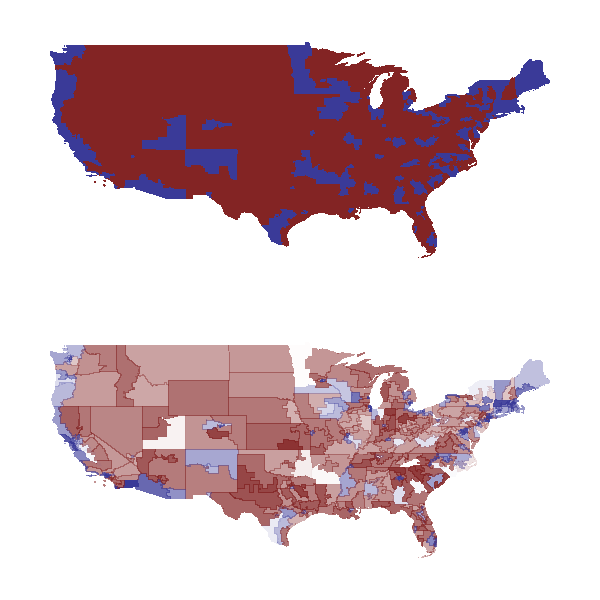
\includegraphics[width=\maxwidth]{figure/data2map} 

\end{knitrout}

All told it took about 13 required lines of code\sidenote{Including lines that just load packages, which technically could all be done in one line.} to go from nothing to a point where I was ready for final mapping, and that includes dropping out Obama's and replacement votes a couple other minor manipulations to make the data fully compatible.  I was able to easily extract points of interest from various objects, manipulate multiple data sets and easily bounce back and forth among them, make changes to them on the fly, import map objects immediately ready for visualization and customization, and take the output from completely independent packages to produce a final product.  Also, I have no formal training or background in political science or GIS mapping, though R has allowed me to play with many tools that such disciplines utilize.

\section{Enhancement}

But what if  you want a little more from this? Say you want to grab the last 10 Congresses?  In R you wouldn't need an explicit loop to do this.  The following code would produce a list of 10 rollcall objects, ready for you to examine whichever one you wanted to at anytime.  The first line creates a vector of appropriate urls, the next feeds them to the readKH function.

\begin{knitrout}\footnotesize
\definecolor{shadecolor}{rgb}{0.969, 0.969, 0.969}\color{fgcolor}\begin{kframe}
\begin{alltt}
\hlstd{congress} \hlkwb{=} \hlkwd{paste0}\hlstd{(}\hlstr{'ftp://voteview.com/hou'}\hlstd{,} \hlnum{103}\hlopt{:}\hlnum{112}\hlstd{,} \hlstr{'kh.ord'}\hlstd{)}
\hlstd{cong103_112} \hlkwb{=} \hlkwd{sapply}\hlstd{(congress, readKH,} \hlkwc{simplify}\hlstd{=F)}
\end{alltt}
\end{kframe}
\end{knitrout}

This takes a few seconds per file, but it's easy to do in parallel with the \emph{\textcolor{blue}{parallel}} package\sidenote{No purchase of a non-crippled version of the software or additional module required.}. If you have your cluster \texttt{clus} setup, just change the second line to the following.


\begin{knitrout}\footnotesize
\definecolor{shadecolor}{rgb}{0.969, 0.969, 0.969}\color{fgcolor}\begin{kframe}
\begin{alltt}
\hlstd{cong103_112} \hlkwb{=} \hlkwd{parSapply}\hlstd{(clus, congress, readKH,} \hlkwc{simplify}\hlstd{=F)}
\end{alltt}
\end{kframe}
\end{knitrout}

I created at function that takes this approach to get either House or Senate (or both), automatically generates descriptions, can write out the file results, and does the process in parallel to create either a rollcall class object or a binary matrix where 1 is a yes vote and 0 a no vote.   You can examine it \href{https://github.com/mclark--/Miscellaneous-R-Code/blob/master/Other/getRollCall.R}{here}.  On my own machine, it would download and create rollcall objects for all legislatures in about twice the time it takes to download just those 10 using the approach above, plus you'd have the other options available.  It also wouldn't take much to add the model and maps as far as code goes, but the models do take several minutes for the House.





% !Rnw root = DDR.Rnw


\part{R for Psychology}
Psychological methodologists jumped on the R bandwagon early, and now have a very wide range of tools to work with from \href{http://cran.r-project.org/web/views/SocialSciences.html}{social sciences} broadly speaking, to \href{http://cran.r-project.org/web/views/Psychometrics.html}{psychometrics} specifically, and others that would be of notable interest such as \href{http://cran.r-project.org/web/views/Multivariate.html}{multivariate analysis}, \href{http://cran.r-project.org/web/views/ExperimentalDesign.html}{experimental design}, \href{http://cran.r-project.org/web/views/MetaAnalysis.html}{meta-analysis}, and even \href{http://cran.r-project.org/web/views/MedicalImaging.html}{brain imaging}.


\section{Example}
I'll start with a latent variable model, as many psychologists use such models to study the underlying constructs they attempt to measure, such as for personality and clinical diagnoses.  To begin, there are a great many tools in the \emph{\textcolor{blue}{psych}} package\sidenote{I use this package frequently for nicely displayed summary statistics and other data exploration.} to engage in exploratory factor analysis, even beyond the standard way most approach such an analysis.  Furthermore, the author of the package provides a freely available online text in \href{http://personality-project.org/revelle.html}{psychometrics}.

I show an example of some data that has 3 underlying factors.  It takes one line to run the model, summarize it or visualize it (latter not shown).  To extract factor scores or loadings for further processing takes no effort at all. 

\begin{knitrout}\footnotesize
\definecolor{shadecolor}{rgb}{0.969, 0.969, 0.969}\color{fgcolor}\begin{kframe}
\begin{alltt}
\hlkwd{library}\hlstd{(psych)}
\hlstd{standardFA} \hlkwb{=} \hlkwd{fa}\hlstd{(Thurstone,} \hlkwc{nfactors} \hlstd{=} \hlnum{3}\hlstd{)}
\hlkwd{summary}\hlstd{(standardFA)}
\end{alltt}
\begin{verbatim}
## 
## Factor analysis with Call: fa(r = Thurstone, nfactors = 3)
## 
## Test of the hypothesis that 3 factors are sufficient.
## The degrees of freedom for the model is 12  and the objective function was  0.01 
## 
## The root mean square of the residuals (RMSA) is  0.01 
## The df corrected root mean square of the residuals is  0.01 
## 
##  With factor correlations of 
##      MR1  MR2  MR3
## MR1 1.00 0.59 0.54
## MR2 0.59 1.00 0.52
## MR3 0.54 0.52 1.00
\end{verbatim}
\begin{alltt}
\hlkwd{fa.diagram}\hlstd{(standardFA)} \hlcom{# visualize}
\hlstd{faScores} \hlkwb{=} \hlkwd{factor.scores}\hlstd{(Thurstone, standardFA)} \hlcom{# extract factor scores}
\hlstd{faLoadings} \hlkwb{=} \hlkwd{loadings}\hlstd{(standardFA)} \hlcom{# extract the loadings}

\hlcom{# modified version using my own function is shown.}
\hlcom{## cor.plot(standardFA)}
\end{alltt}
\end{kframe}
\end{knitrout}
\marginnote{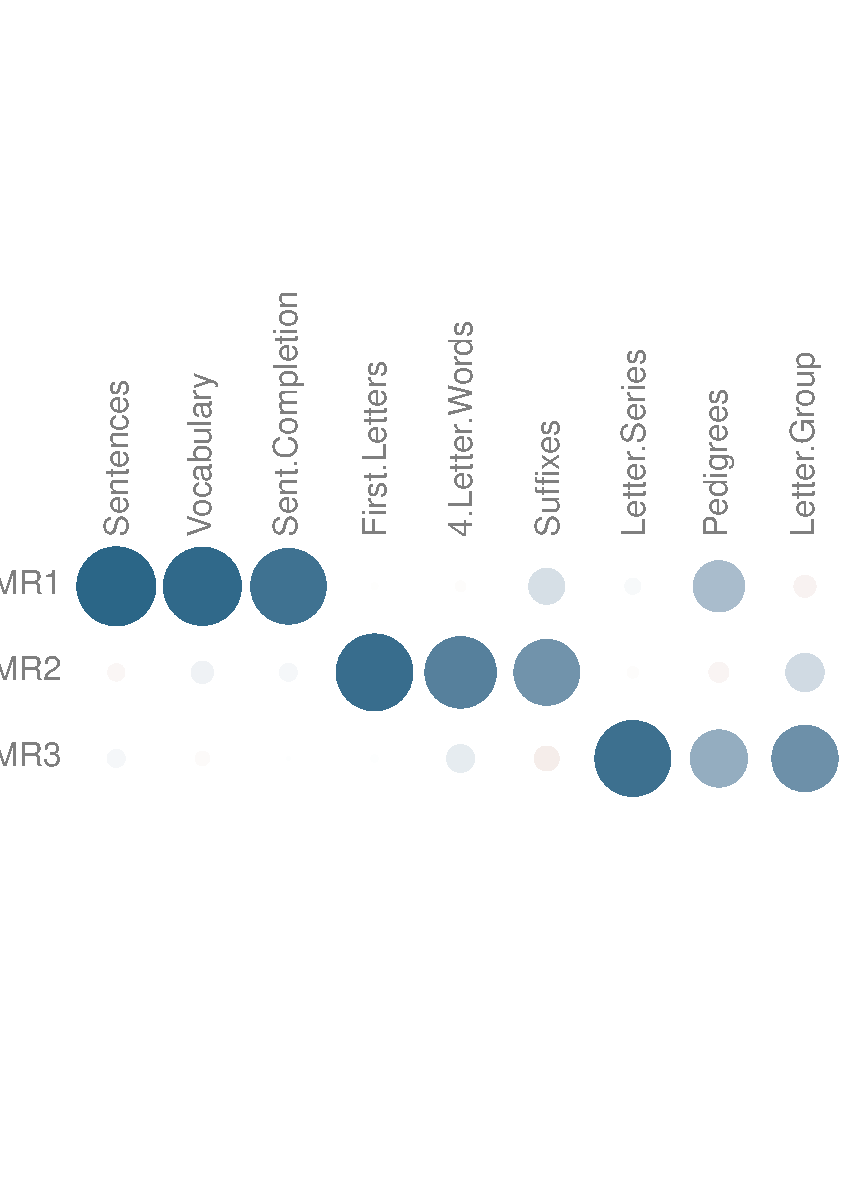
\includegraphics[scale=.375]{loadingPlot}} 
We can see that most items load nicely on 3 correlated factors, but a couple appear to have slight crossloadings on other factors.  

\section{Enhancement}
Let's say I wanted to simply explore the possibility of a hierarchical factor structure. This isn't something I'm sold on, I don't necessarily want to get carried away analytically, just explore.  R allows one to do this sort of thing all the time, because it is easy to extract the pieces of model output you would like for further processing, or simply use other functionality and visualization.  

\begin{knitrout}\footnotesize
\definecolor{shadecolor}{rgb}{0.969, 0.969, 0.969}\color{fgcolor}\begin{kframe}
\begin{alltt}
\hlkwd{omega.diagram}\hlstd{(}\hlkwd{omega}\hlstd{(Thurstone))}
\end{alltt}
\end{kframe}
\end{knitrout}
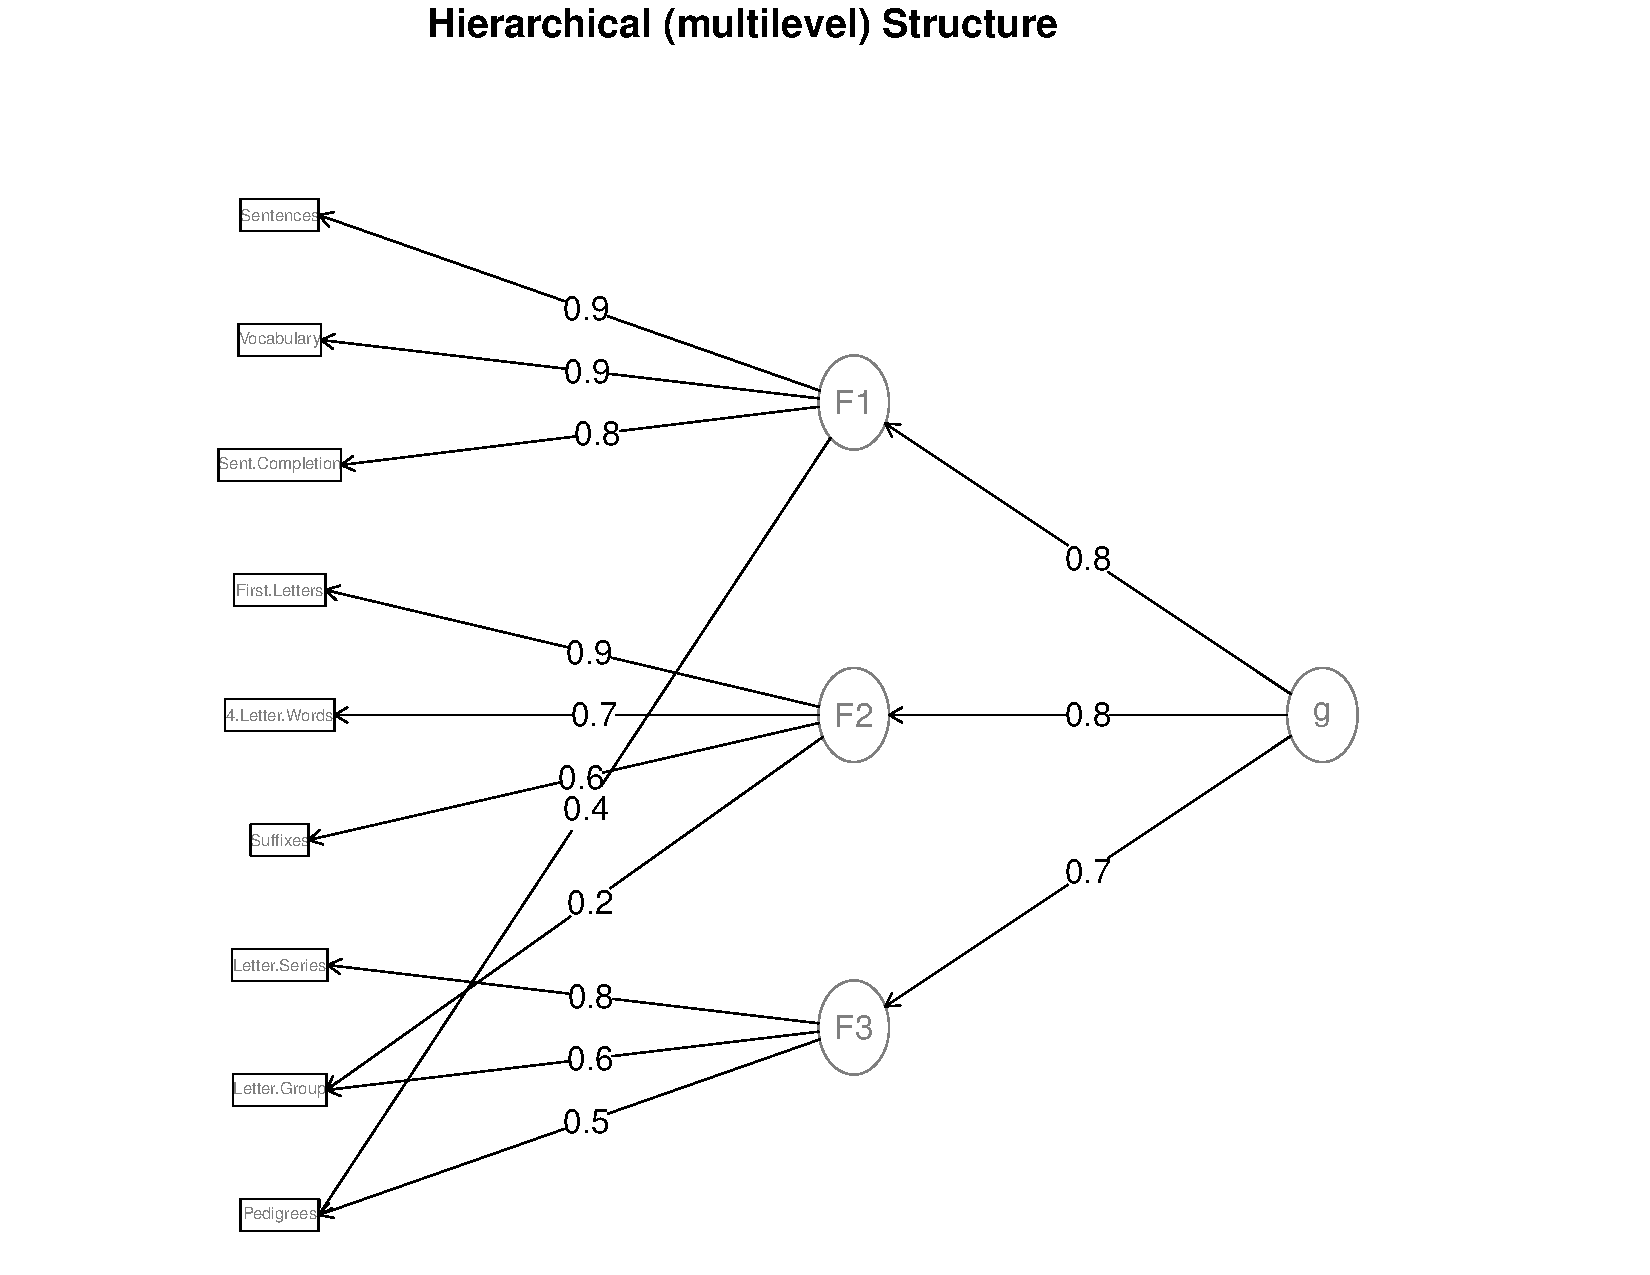
\includegraphics[scale=.4]{FAHierarchical.pdf}

Other tools in this area include the \emph{\textcolor{blue}{MplusAutomation}} package, which will write out different iterations of an Mplus syntax template, run the files in Mplus, extract the output, and provide the summary of all models, \emph{and you never have to leave the R environment}.  However, now you may not even need Mplus. The \emph{\textcolor{blue}{lavaan}} package provides most of the functionality in Mplus as well as output formatted in the same fashion.



% !Rnw root = DDR.Rnw



\part{R for Sociology}
Sociologists have plenty of ways to benefit from using R.  Along with general \href{http://cran.r-project.org/web/views/SocialSciences.html}{social science packages}, there are packages pertaining to \href{http://cran.r-project.org/web/views/OfficialStatistics.html}{official statistics and survey design}, and graphical modeling including \href{http://cran.r-project.org/web/views/gR.html}{social networks}.  I will provide an example of the latter.

\section{Example}
For network analysis there are a great many tools in R such as the packages \emph{\textcolor{blue}{sna}}, \emph{\textcolor{blue}{igraph}} and so forth.  As a simple example we can begin with a data matrix, and from it create an adjacency matrix in which a 1 (or more) represents a connection for two observations, and finally plot the network graph.

Let's say we have a data set for 10 individuals and 6 individuals.  First we take a look.

\begin{knitrout}\footnotesize
\definecolor{shadecolor}{rgb}{0.969, 0.969, 0.969}\color{fgcolor}\begin{kframe}
\begin{alltt}
\hlkwd{colnames}\hlstd{(snData)} \hlkwb{=} \hlkwd{paste0}\hlstd{(}\hlstr{'V'}\hlstd{,}\hlnum{1}\hlopt{:}\hlnum{6}\hlstd{)}
\hlstd{snData}
\end{alltt}
\begin{verbatim}
##            V1  V2  V3  V4 V5  V6
## Yelberton  No  No  No  No No  No
## Billy      No  No  No  No No  No
## Fred       No  No  No  No No  No
## Henrietta  No Yes  No  No No  No
## Janie     Yes  No  No  No No  No
## Bertha     No Yes Yes  No No  No
## Willie     No  No  No  No No  No
## Iggy       No  No Yes  No No  No
## Flozelle   No  No Yes Yes No  No
## Louise     No  No  No Yes No Yes
\end{verbatim}
\end{kframe}
\end{knitrout}

For our purposes, let's say that if anyone has 'Yes' as a value for a particular variable, then, based on that, individuals are connected to anyone else with a 'Yes', and more so the more variables in which this occurs. Now there various distance metrics we could employ for such data that would only take a single line of code to create an adjacency/distance matrix (e.g. binary distance, Hamming's distance etc.).  For demonstration though, we'll do it ourselves.  

For a moment you might think about how you would go about this in a standard statistics package.  I can imagine your thoughts might take you through a double loop to calculate adjacency, figure out where to store or write out the matrix, do all this as a completely separate enterprise, then bring in your matrix to possibly another specialized package entirely that can better handle such things.  This is an area traditional statistical packages have only recently begun to even offer much regarding, but regardless there would be a number of steps

In the following, I create an object containing all possible pairwise connections among the rows 1 through 10. I then make an empty matrix that will eventually become the adjacency matrix. In one line of code I'm able make the all calculations by implicitly creating my own function that will sum all occasions in which both inputs are 'yes', and this is applied to the object with all the pairwise combinations, whose elements serve as a row index for the original matrix.  I then fill in the lower triangle of the matrix with those values, and as a shortcut, use the dist function (for distance matrices) to fill in the rest.


\begin{knitrout}\footnotesize
\definecolor{shadecolor}{rgb}{0.969, 0.969, 0.969}\color{fgcolor}\begin{kframe}
\begin{alltt}
\hlstd{pairwise} \hlkwb{=} \hlkwd{combn}\hlstd{(}\hlkwd{nrow}\hlstd{(snData),} \hlnum{2}\hlstd{)}
\hlstd{adjmat} \hlkwb{=} \hlkwd{matrix}\hlstd{(}\hlnum{NA}\hlstd{,} \hlnum{10}\hlstd{,} \hlnum{10}\hlstd{)}
\hlstd{adj} \hlkwb{=} \hlkwd{apply}\hlstd{(pairwise,} \hlnum{2}\hlstd{,} \hlkwa{function}\hlstd{(}\hlkwc{x}\hlstd{)} \hlkwd{sum}\hlstd{(snData[x[}\hlnum{1}\hlstd{],]}\hlopt{==}\hlstr{'Yes'} \hlopt{&} \hlstd{snData[x[}\hlnum{2}\hlstd{],]}\hlopt{==}\hlstr{'Yes'}\hlstd{))}
\hlstd{adjmat[}\hlkwd{lower.tri}\hlstd{(adjmat)]} \hlkwb{=} \hlstd{adj}
\hlstd{adjmat} \hlkwb{=} \hlkwd{as.matrix}\hlstd{(}\hlkwd{as.dist}\hlstd{(adjmat,} \hlkwc{diag}\hlstd{=T,} \hlkwc{upper}\hlstd{=T))}
\hlstd{adjmat}
\end{alltt}
\begin{verbatim}
##           Yelberton Billy Fred Henrietta Janie Bertha Willie Iggy Flozelle Louise
## Yelberton         0     0    0         0     0      0      0    0        0      0
## Billy             0     0    0         0     0      0      0    0        0      0
## Fred              0     0    0         0     0      0      0    0        0      0
## Henrietta         0     0    0         0     0      1      0    0        0      0
## Janie             0     0    0         0     0      0      0    0        0      0
## Bertha            0     0    0         1     0      0      0    1        1      0
## Willie            0     0    0         0     0      0      0    0        0      0
## Iggy              0     0    0         0     0      1      0    0        1      0
## Flozelle          0     0    0         0     0      1      0    1        0      1
## Louise            0     0    0         0     0      0      0    0        1      0
\end{verbatim}
\end{kframe}
\end{knitrout}


\noindent Now we can plot the graph.  The plot shown has some additional arguments added.


\begin{knitrout}\footnotesize
\definecolor{shadecolor}{rgb}{0.969, 0.969, 0.969}\color{fgcolor}\begin{kframe}
\begin{alltt}
\hlkwd{library}\hlstd{(igraph)}
\hlstd{g} \hlkwb{=} \hlkwd{graph.adjacency}\hlstd{(adjmat)}
\hlkwd{plot}\hlstd{(g)}
\end{alltt}
\end{kframe}
\end{knitrout}
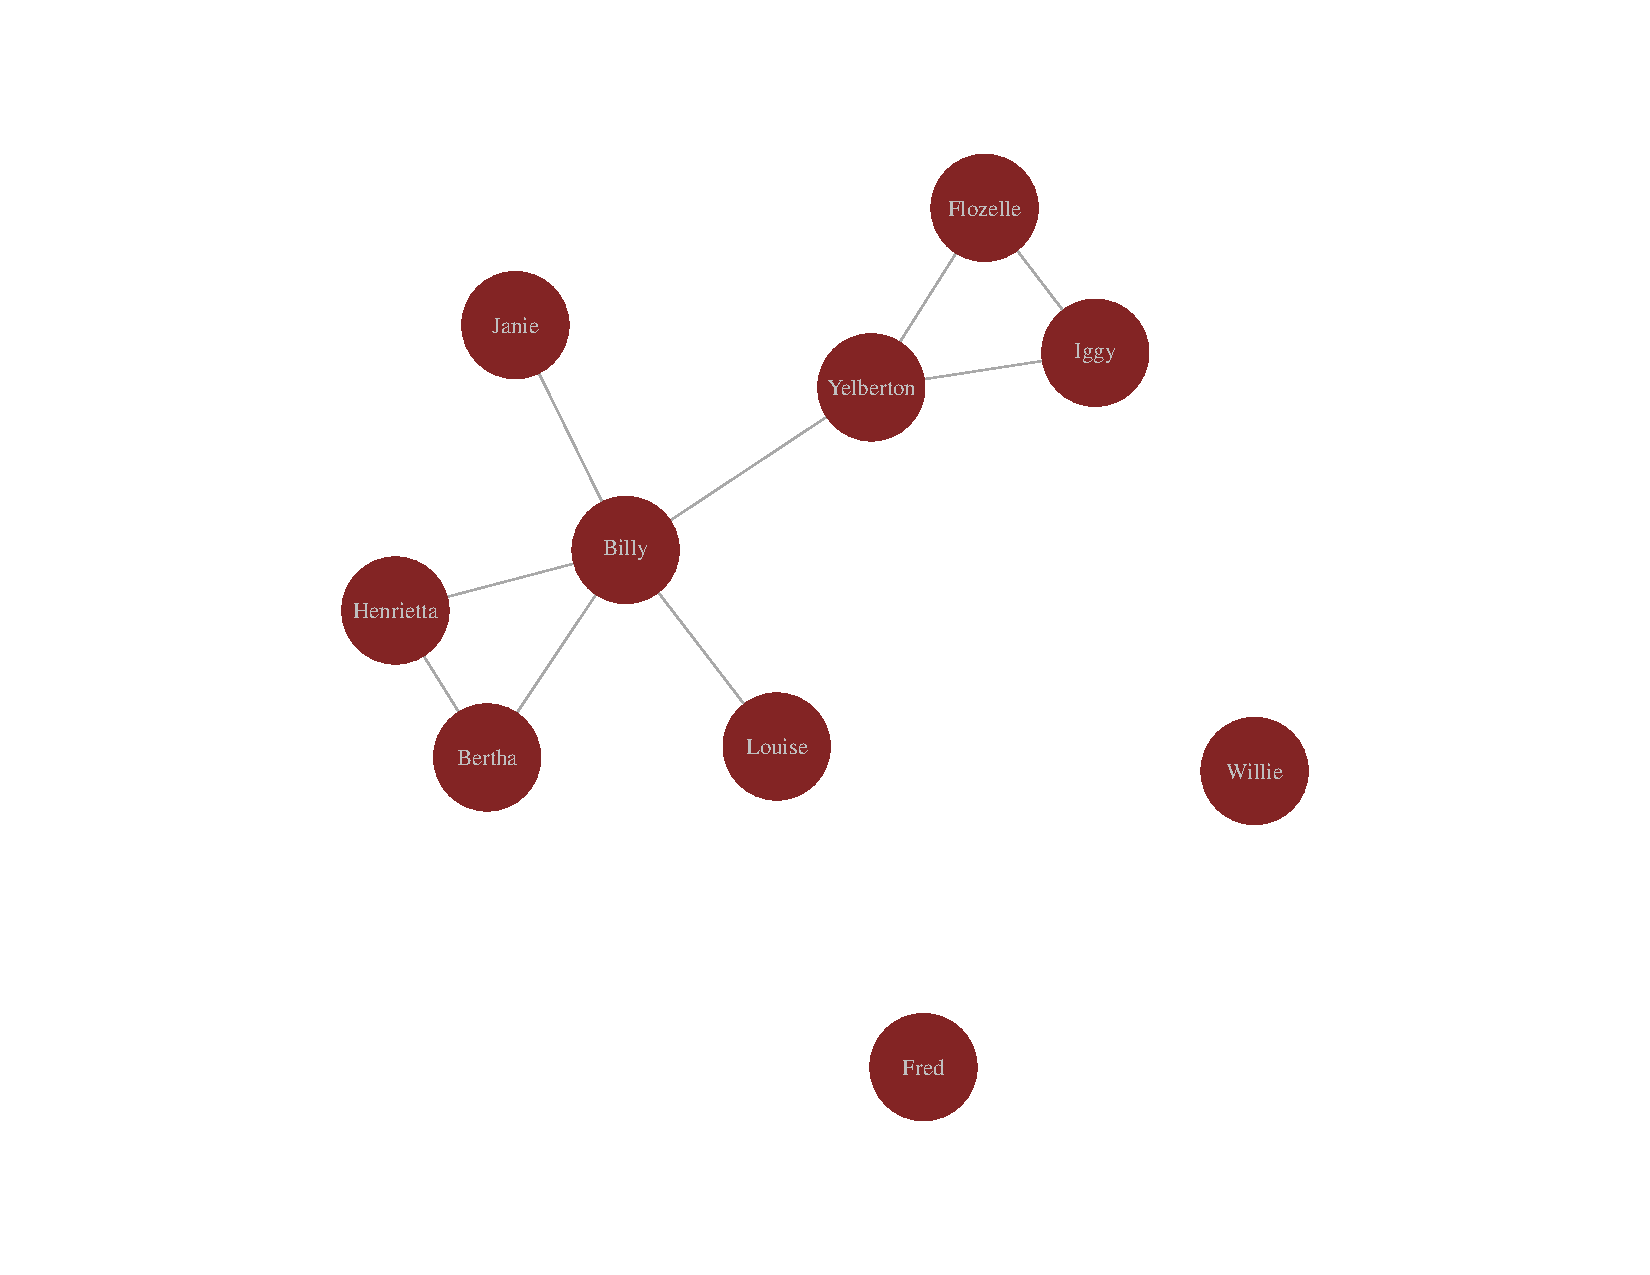
\includegraphics[scale=.38]{networkgraph}


Note that we were able to not only able to do this efficiently in our code, we never had leave the current R environment, use multiple data files or multiple programs, and we have plenty enough functionality to calculate network metrics and model the network itself.  We also have code that would be trivial to change to other parameters of determining adjacency.

\section{Enhancement}
What if you want more?  Maybe you want to put an interactive, force-directed graph of the network on your website.  The following code will create the html you need, at which point you can either use it directly as a webpage or embed it in another.  The interactive version is \href{http://www3.nd.edu/~mclark19/misc/demos/network.html}{here}; click to add a name and change the color.

\begin{knitrout}\footnotesize
\definecolor{shadecolor}{rgb}{0.969, 0.969, 0.969}\color{fgcolor}\begin{kframe}
\begin{alltt}
\hlkwd{library}\hlstd{(d3Network)}
\hlkwd{d3SimpleNetwork}\hlstd{(}\hlkwd{data.frame}\hlstd{(}\hlkwd{get.edgelist}\hlstd{(g)),} \hlkwc{file}\hlstd{=}\hlstr{'network.html'}\hlstd{)}
\end{alltt}
\end{kframe}
\end{knitrout}
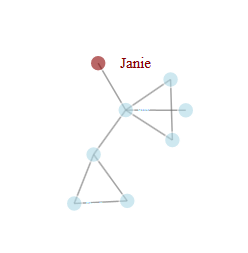
\includegraphics[scale=.9]{d3network}


% !Rnw root = DDR.Rnw



\part{Brief Summary}
At this point we've seen R in action in engaged in typical social science data and methodological activity.  We've also seen that it can be very easy to take the process further, and generally, that's how it is with R.  You get a feel for things, and then realize the potential, take your process further.  It allows for far easier data exploration\sidenote{Let's say you had a list object containing 1000 simulated data sets and you wanted to run a model on each. This would take one line of code in R.  Let's say you wanted to run 1000 separate models on each data set.  Assuming a corresponding list of formulas specifying the models, this too would take one line of code.}, allows one to easily specify and compare the output from alternative models, and use that for visualization.

What might not have been obvious is how easily the different packages work with the objects you create.  The packages might be created by different people, but they work on the same classes of R objects, and so many of them work very much in the same fashion even for quite different goals. But even for different classes of objects, different methods for the same function will produce a different product for an object of a different class.  

One might also make the claim 'Yeah but, you already know R, I couldn't have done those things!'.  And that's where you'd be incorrect.  There is so much information about R on the web and elsewhere with working demonstrations and usable code that you merely have to find who else did something, and tweak it for your own needs\sidenote{For the state naming issue, I hadn't done that before, but in looking for an R function that created state abbreviations, I came acros a stack overflow example.}.  

In the following I'll show how to do common tasks such as import data, get basic descriptive statistics and visuals, and run traditional models.  The point will be to show how easy it is to use R just as you would SAS, SPSS or Stata for common tasks irrespective of discipline or analysis.  For most of those things it would take very little transition time if you've done any programming in another language.



% !Rnw root = DDR.Rnw



\part{Working with Data}

It is no more difficult to get data into R than other programs.  The following offer different ways to read in data in standard formats and from common statistical packages.

\begin{knitrout}\footnotesize
\definecolor{shadecolor}{rgb}{0.969, 0.969, 0.969}\color{fgcolor}\begin{kframe}
\begin{alltt}
\hlstd{myCsvDatainR} \hlkwb{=} \hlkwd{read.csv}\hlstd{(}\hlstr{'mydata.csv'}\hlstd{)}
\hlstd{myTabDelimDatainR} \hlkwb{=} \hlkwd{read.table}\hlstd{(}\hlstr{'mydata.dat'}\hlstd{)}

\hlcom{# for statistical packages}
\hlkwd{library}\hlstd{(foreign)}

\hlstd{mySPSSDatainR} \hlkwb{=} \hlkwd{read.spss}\hlstd{(}\hlstr{'mydata.sav'}\hlstd{)}
\hlstd{myStataDatainR} \hlkwb{=} \hlkwd{read.dta}\hlstd{(}\hlstr{'mydata.dta'}\hlstd{)}
\end{alltt}
\end{kframe}
\end{knitrout}

Probably one of the most powerful advantages R has over other statistical packages is its indexing capabilities.  To provide an arbitrary but extreme example, I will subset a data set as follows: if the fitted value from a regression (R object \texttt{modlm}) is above 10 and, following that, if Sex is male or their Mood, which is in another data set (mydata2), is 'blue', but only the variables whose name begins with 'Alf' or ends with 'Webster', and we only want to keep the last 10 rows, and finally, we want summary statistics for those that are retained. Note that none of these particular variables are already available except those in the data sets.  Think of the ways in which you might accomplish this in your statistical package of choice.  Mostly it would involve steps to create the fitted values, create the conditional variables, create a variable list, run the initial conditionals, subset to the last 10 rows, and finally run a separate command to summarize the output.  In the following, we're going to do all of this on the fly. 


\begin{knitrout}\footnotesize
\definecolor{shadecolor}{rgb}{0.969, 0.969, 0.969}\color{fgcolor}\begin{kframe}
\begin{alltt}
\hlstd{subsetData} \hlkwb{=} \hlkwd{summary}\hlstd{(}\hlkwd{tail}\hlstd{(mydata[}\hlkwd{fitted}\hlstd{(modlm)}\hlopt{>}\hlnum{10} \hlopt{&&} \hlstd{mydata}\hlopt{$}\hlstd{Sex}\hlopt{==}\hlstr{'male'} \hlopt{|} \hlstd{mydata2}\hlopt{$}\hlstd{Mood}\hlopt{==}\hlstr{'blue'}\hlstd{,}
                                 \hlkwd{grep}\hlstd{(}\hlstr{'^Alf|Webster$'}\hlstd{,} \hlkwd{colnames}\hlstd{(mydata))],} \hlnum{10}\hlstd{))}
\end{alltt}
\end{kframe}
\end{knitrout}

\emph{\textbf{One line of code}}.  This would be a bad way to code and not recommended due to clarity, but it serves to illustrate a point, namely \emph{that you can}.  Furthermore, once you get used to these capabilities you end up taking advantage of them in ways you just simply wouldn't have thought to do in other statistical packages because it either wouldn't have been possible or would have been overly difficult.  Once you start doing this, data manipulation and exploration, part and parcel of \emph{initial data analysis}, might actually even be fun.  While you might spend weeks cleaning data using traditional stat packages, you'll already have made new discoveries from venturing down paths you otherwise wouldn't have bothered with due to time constraints.

A student or faculty member that only occasionally uses a statistical package from time to time when they have some data they want to analyze in all likelihood doesn't do enough programming to be overly wed to a statistical package, and this is because they likely don't do a lot of advanced programming anyway.  That said, why not instead use one that will save you time in the long run even if you don't use all of its power?

\section{RData}
Another efficiency feature R has over other statistical packages is the RData file itself.  When you save your workspace, you aren't just saving a data set, you are able to save \emph{every object you've created}.  When you load the RData file, \emph{you don't even have to rerun any code}. All objects are available, including graphs if saved as objects.  Even if one could program as flexibly in another statistical package, in those you'd always have to reimport data and rerun code to get back to the point you were. R allows you to pick up at the exact point you left off.


% !Rnw root = DDR.Rnw



\part{Models}

Let's start by examining some non-R approaches to the basic modeling case of standard regression.
\bigskip

\noindent SPSS
\begin{footnotesize}
\begin{verbatim}
regression
 /dependent science
 /method = enter math female socst read.
\end{verbatim}
\end{footnotesize}

\noindent SAS
\begin{footnotesize}
\begin{verbatim}
proc reg;
model science = math female socst read;
run;
\end{verbatim}
\end{footnotesize}

\noindent Stata
\begin{footnotesize}
\begin{verbatim}
reg science math female socst read
\end{verbatim}
\end{footnotesize}

\noindent R
\begin{footnotesize}
\begin{verbatim}
lm(science ~ math + female + socst + read)
\end{verbatim}
\end{footnotesize}
This is as basic as modeling gets, and maybe it's just me, but as far as code goes, even in this simple setting I think most would prefer the latter two for their legibility and efficiency\sidenote{Though unless you know Stata, you wouldn't necessarily know what model is being run.}. The following are some standard models in the social sciences in R code.

\begin{knitrout}\footnotesize
\definecolor{shadecolor}{rgb}{0.969, 0.969, 0.969}\color{fgcolor}\begin{kframe}
\begin{alltt}
\hlcom{# standard linear model regression}
\hlkwd{lm}\hlstd{(y} \hlopt{~} \hlstd{x1} \hlopt{+} \hlstd{x2)}

\hlcom{# generalized linear model (poisson)}
\hlkwd{glm}\hlstd{(y} \hlopt{~} \hlstd{x1} \hlopt{+} \hlstd{x2,} \hlkwc{family}\hlstd{=}\hlstr{'poisson'}\hlstd{)}

\hlcom{# mixed model, random intercept (lme4 package)}
\hlkwd{lmer}\hlstd{(y} \hlopt{~} \hlstd{x1} \hlopt{+} \hlstd{x2} \hlopt{+} \hlstd{(}\hlnum{1}\hlopt{|}\hlstd{group))}

\hlcom{# generlized mixed model (with a random slope added)}
\hlkwd{glmer}\hlstd{(y} \hlopt{~} \hlstd{x1} \hlopt{+} \hlstd{x2} \hlopt{+} \hlstd{(}\hlnum{1} \hlopt{+} \hlstd{x1}\hlopt{|}\hlstd{group),} \hlkwc{family}\hlstd{=}\hlstr{'poisson'}\hlstd{)}

\hlcom{# survival model}
\hlkwd{coxph}\hlstd{(}\hlkwd{Surv}\hlstd{(time, status)} \hlopt{~} \hlstd{x1} \hlopt{+} \hlstd{x2)}

\hlcom{# principal components}
\hlkwd{princomp}\hlstd{(mydata)}
\end{alltt}
\end{kframe}
\end{knitrout}

Hopefully the general theme is clear.  After data manipulation running a typical model in R is just as or even more easy to do in R, typically one needs to just specify a formula object (i.e. y\textasciitilde x) and note the data (if the variables are not otherwise in the environment).  But let's look at what we might do with a standard regression. The following runs a simple model and shows the results.

\begin{knitrout}\footnotesize
\definecolor{shadecolor}{rgb}{0.969, 0.969, 0.969}\color{fgcolor}\begin{kframe}
\begin{alltt}
\hlstd{modlm} \hlkwb{=} \hlkwd{lm}\hlstd{(y} \hlopt{~} \hlstd{x1} \hlopt{+} \hlstd{x2,} \hlkwc{data}\hlstd{=mydata)}
\hlkwd{summary}\hlstd{(modlm)}
\end{alltt}
\begin{verbatim}
## 
## Call:
## lm(formula = y ~ x1 + x2, data = mydata)
## 
## Residuals:
##     Min      1Q  Median      3Q     Max 
## -2.9985 -0.5104  0.0139  0.5602  2.7546 
## 
## Coefficients:
##             Estimate Std. Error t value Pr(>|t|)    
## (Intercept)   0.1000     0.0592    1.69  0.09261 .  
## x1            0.2000     0.0593    3.37  0.00087 ***
## x2            0.3000     0.0593    5.05  8.4e-07 ***
## ---
## Signif. codes:  0 '***' 0.001 '**' 0.01 '*' 0.05 '.' 0.1 ' ' 1
## 
## Residual standard error: 0.937 on 247 degrees of freedom
## Multiple R-squared:  0.13,	Adjusted R-squared:  0.123 
## F-statistic: 18.5 on 2 and 247 DF,  p-value: 3.39e-08
\end{verbatim}
\end{kframe}
\end{knitrout}

But it's not enough to merely get results.  Every model must be examined to see how well it fits the data, how tenable assumptions are etc.  It also aids interpretation to see predictive plots and so forth. A set of diagnostic plots is readily available in for many standard models by simply using the \texttt{\textcolor{red}{plot}} function on the lm object.

\begin{knitrout}\footnotesize
\definecolor{shadecolor}{rgb}{0.969, 0.969, 0.969}\color{fgcolor}\begin{kframe}
\begin{alltt}
\hlkwd{plot}\hlstd{(modlm,} \hlkwc{ask}\hlstd{=F)}
\end{alltt}
\end{kframe}
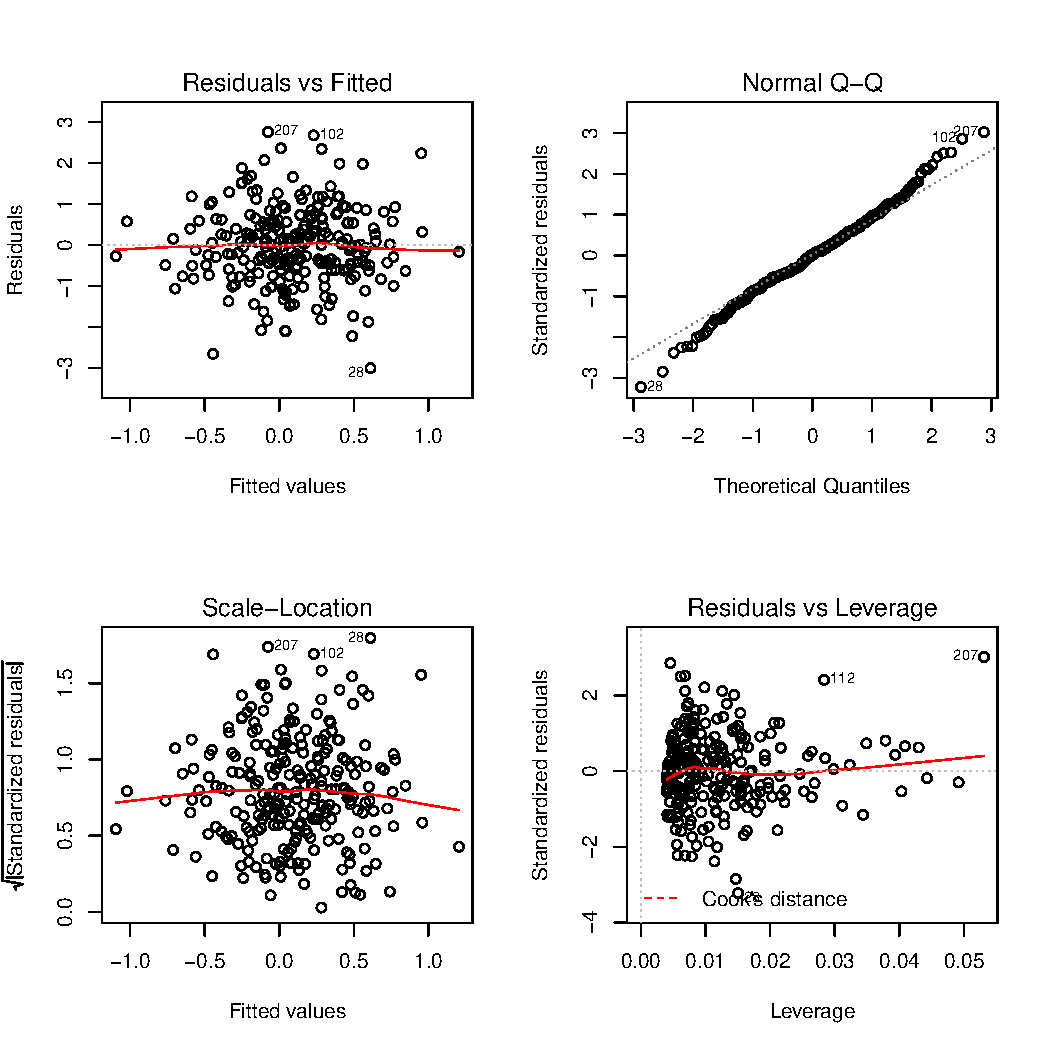
\includegraphics[width=\maxwidth]{figure/lmResiduals} 

\end{knitrout}

\noindent Or do it yourself.

\begin{knitrout}\footnotesize
\definecolor{shadecolor}{rgb}{0.969, 0.969, 0.969}\color{fgcolor}\begin{kframe}
\begin{alltt}
\hlkwd{plot}\hlstd{(modlm}\hlopt{$}\hlstd{fitted, modlm}\hlopt{$}\hlstd{residuals)}
\end{alltt}
\end{kframe}
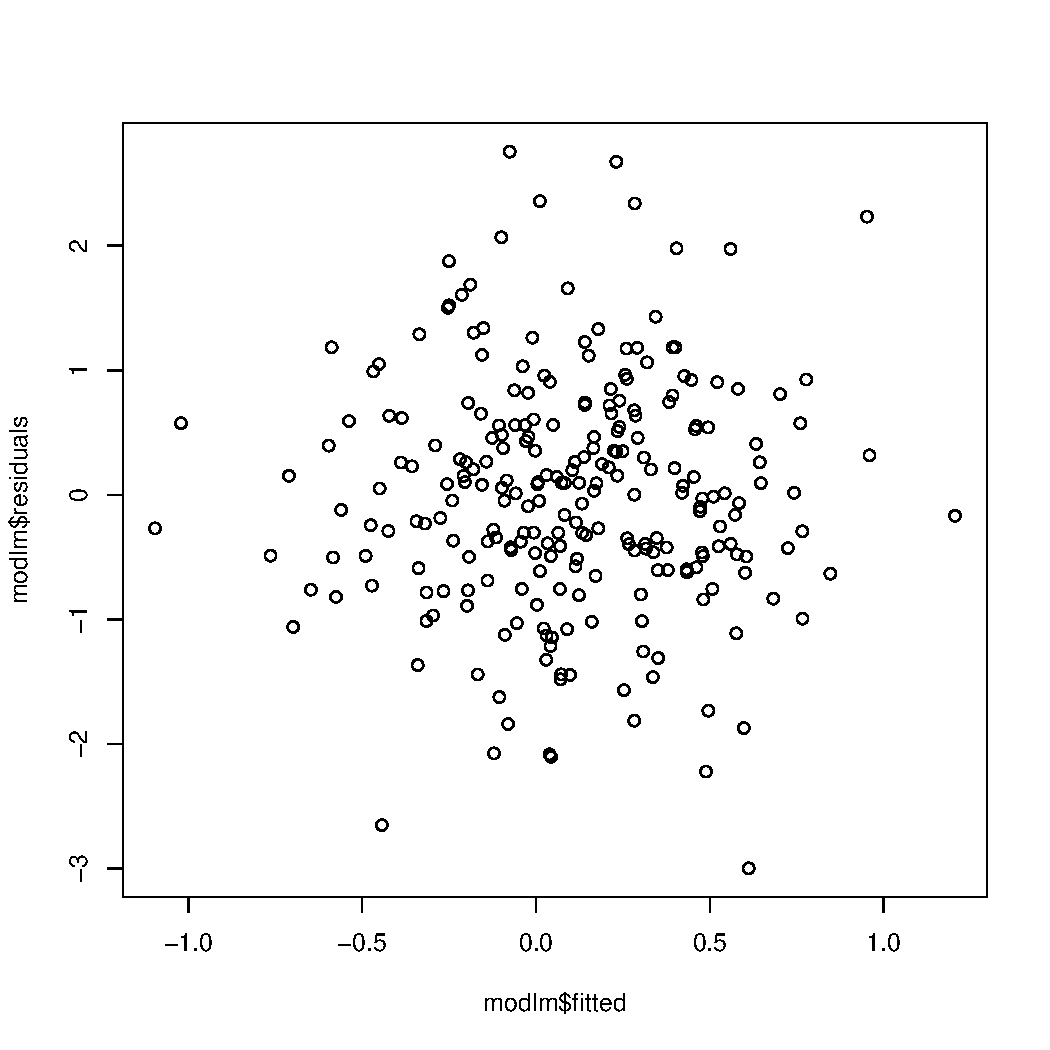
\includegraphics[width=.49\linewidth]{figure/lmresplot} 

\end{knitrout}


Note that in the first place we have several diagnostics ready to go for all lm, glm, and additive models, as well as many others in various packages. R developers know you need these sorts of things and so make it easy to get, but even then R objects make it easy to extract them for your own purposes.  The following shows everything that can be extracted from the model object such as coefficients, model matrix, residuals etc.  You can extract other things from the summary object (not shown).

\begin{knitrout}\tiny
\definecolor{shadecolor}{rgb}{0.969, 0.969, 0.969}\color{fgcolor}\begin{kframe}
\begin{alltt}
\hlkwd{str}\hlstd{(modlm)}
\hlcom{## str(summary(modlm))}
\end{alltt}
\begin{verbatim}
## List of 12
##  $ coefficients : Named num [1:3] 0.1 0.2 0.3
##   ..- attr(*, "names")= chr [1:3] "(Intercept)" "x1" "x2"
##  $ residuals    : Named num [1:250] 0.964 0.086 0.344 0.395 0.818 ...
##   ..- attr(*, "names")= chr [1:250] "1" "2" "3" "4" ...
##  $ effects      : Named num [1:250] -1.581 3.156 4.734 0.305 0.739 ...
##   ..- attr(*, "names")= chr [1:250] "(Intercept)" "x1" "x2" "" ...
##  $ rank         : int 3
##  $ fitted.values: Named num [1:250] 0.2563 -0.2559 0.2314 -0.596 -0.0228 ...
##   ..- attr(*, "names")= chr [1:250] "1" "2" "3" "4" ...
##  $ assign       : int [1:3] 0 1 2
##  $ qr           :List of 5
##   ..$ qr   : num [1:250, 1:3] -15.8114 0.0632 0.0632 0.0632 0.0632 ...
##   .. ..- attr(*, "dimnames")=List of 2
##   .. .. ..$ : chr [1:250] "1" "2" "3" "4" ...
##   .. .. ..$ : chr [1:3] "(Intercept)" "x1" "x2"
##   .. ..- attr(*, "assign")= int [1:3] 0 1 2
##   ..$ qraux: num [1:3] 1.06 1.01 1.02
##   ..$ pivot: int [1:3] 1 2 3
##   ..$ tol  : num 1e-07
##   ..$ rank : int 3
##   ..- attr(*, "class")= chr "qr"
##  $ df.residual  : int 247
##  $ xlevels      : Named list()
##  $ call         : language lm(formula = y ~ x1 + x2, data = mydata)
##  $ terms        :Classes 'terms', 'formula' length 3 y ~ x1 + x2
##   .. ..- attr(*, "variables")= language list(y, x1, x2)
##   .. ..- attr(*, "factors")= int [1:3, 1:2] 0 1 0 0 0 1
##   .. .. ..- attr(*, "dimnames")=List of 2
##   .. .. .. ..$ : chr [1:3] "y" "x1" "x2"
##   .. .. .. ..$ : chr [1:2] "x1" "x2"
##   .. ..- attr(*, "term.labels")= chr [1:2] "x1" "x2"
##   .. ..- attr(*, "order")= int [1:2] 1 1
##   .. ..- attr(*, "intercept")= int 1
##   .. ..- attr(*, "response")= int 1
##   .. ..- attr(*, ".Environment")=<environment: R_GlobalEnv> 
##   .. ..- attr(*, "predvars")= language list(y, x1, x2)
##   .. ..- attr(*, "dataClasses")= Named chr [1:3] "numeric" "numeric" "numeric"
##   .. .. ..- attr(*, "names")= chr [1:3] "y" "x1" "x2"
##  $ model        :'data.frame':	250 obs. of  3 variables:
##   ..$ y : num [1:250] 1.22 -0.17 0.576 -0.201 0.795 ...
##   ..$ x1: num [1:250] -0.495 -0.253 0.931 -0.886 1.231 ...
##   ..$ x2: num [1:250] 0.851 -1.018 -0.183 -1.729 -1.23 ...
##   ..- attr(*, "terms")=Classes 'terms', 'formula' length 3 y ~ x1 + x2
##   .. .. ..- attr(*, "variables")= language list(y, x1, x2)
##   .. .. ..- attr(*, "factors")= int [1:3, 1:2] 0 1 0 0 0 1
##   .. .. .. ..- attr(*, "dimnames")=List of 2
##   .. .. .. .. ..$ : chr [1:3] "y" "x1" "x2"
##   .. .. .. .. ..$ : chr [1:2] "x1" "x2"
##   .. .. ..- attr(*, "term.labels")= chr [1:2] "x1" "x2"
##   .. .. ..- attr(*, "order")= int [1:2] 1 1
##   .. .. ..- attr(*, "intercept")= int 1
##   .. .. ..- attr(*, "response")= int 1
##   .. .. ..- attr(*, ".Environment")=<environment: R_GlobalEnv> 
##   .. .. ..- attr(*, "predvars")= language list(y, x1, x2)
##   .. .. ..- attr(*, "dataClasses")= Named chr [1:3] "numeric" "numeric" "numeric"
##   .. .. .. ..- attr(*, "names")= chr [1:3] "y" "x1" "x2"
##  - attr(*, "class")= chr "lm"
\end{verbatim}
\end{kframe}
\end{knitrout}


Prediction is straightforward, and works the same in many modeling packages.  Again, R developers know this is part and parcel of statistical analysis, and it is made easy for standard models, and most modeling packages take the same approach.  In the following we merely have to tell it what values of the explanatory variables you want to use\sidenote{If you didn't you'd just be duplicating the fitted values.}.  Here we look at x1 values from -1 to 1, keeping x2 at its 90th percentile.  Note that we aren't explicitly creating new x1 or x2 variables, though it would be better form to create a separate 'newdata' object


\begin{knitrout}\footnotesize
\definecolor{shadecolor}{rgb}{0.969, 0.969, 0.969}\color{fgcolor}\begin{kframe}
\begin{alltt}
\hlkwd{predict}\hlstd{(modlm,} \hlkwd{data.frame}\hlstd{(}\hlkwc{x1}\hlstd{=}\hlkwd{seq}\hlstd{(}\hlopt{-}\hlnum{1}\hlstd{,}\hlnum{1}\hlstd{,} \hlkwc{by}\hlstd{=}\hlnum{.25}\hlstd{),} \hlkwc{x2}\hlstd{=}\hlkwd{quantile}\hlstd{(mydata}\hlopt{$}\hlstd{x2,} \hlkwc{p}\hlstd{=}\hlnum{.9}\hlstd{)))}
\end{alltt}
\begin{verbatim}
##      1      2      3      4      5      6      7      8      9 
## 0.2901 0.3401 0.3901 0.4401 0.4901 0.5401 0.5901 0.6401 0.6901
\end{verbatim}
\end{kframe}
\end{knitrout}

\noindent Here are some examples of other typical modeling exercises.

\begin{knitrout}\footnotesize
\definecolor{shadecolor}{rgb}{0.969, 0.969, 0.969}\color{fgcolor}\begin{kframe}
\begin{alltt}
\hlcom{# interactions (including main effects)}
\hlkwd{lm}\hlstd{(y} \hlopt{~} \hlstd{x1}\hlopt{*}\hlstd{x2)}

\hlcom{# dealing with categorical factors; nothing special needed}
\hlkwd{lm}\hlstd{(y} \hlopt{~} \hlstd{f1} \hlopt{+} \hlstd{x2)}

\hlcom{# transform a variable on the fly; no need to explicitly create the variables if}
\hlcom{# you don't want to. The last one creates a logical variable that's true if x is}
\hlcom{# greater than 5.}
\hlkwd{lm}\hlstd{(}\hlkwd{log}\hlstd{(y)} \hlopt{~} \hlkwd{sqrt}\hlstd{(x1)} \hlopt{+} \hlstd{x2}\hlopt{>}\hlnum{5}\hlstd{)}

\hlcom{# add a predictor}
\hlkwd{update}\hlstd{(modlm,} \hlopt{~}\hlstd{.} \hlopt{+} \hlstd{x3)}

\hlcom{# model comparsion}
\hlkwd{anova}\hlstd{(mod1, mod2)}

\hlcom{# automatic model comparison of added or dropped terms}
\hlkwd{drop1}\hlstd{(modlm,} \hlopt{~} \hlstd{x2,} \hlkwc{test}\hlstd{=}\hlstr{'Chisq'}\hlstd{)}
\hlkwd{add1}\hlstd{(modlm,} \hlopt{~} \hlstd{x1}\hlopt{*}\hlstd{x2,} \hlkwc{test}\hlstd{=}\hlstr{'Chisq'}\hlstd{)}

\hlcom{# y predicted by all other variables}
\hlkwd{lm}\hlstd{(y} \hlopt{~} \hlstd{.)}

\hlcom{# write out results to latex (xtable package)}
\hlkwd{xtable}\hlstd{(}\hlkwd{summary}\hlstd{(modlm))}
\end{alltt}
\end{kframe}
\end{knitrout}
\marginnote{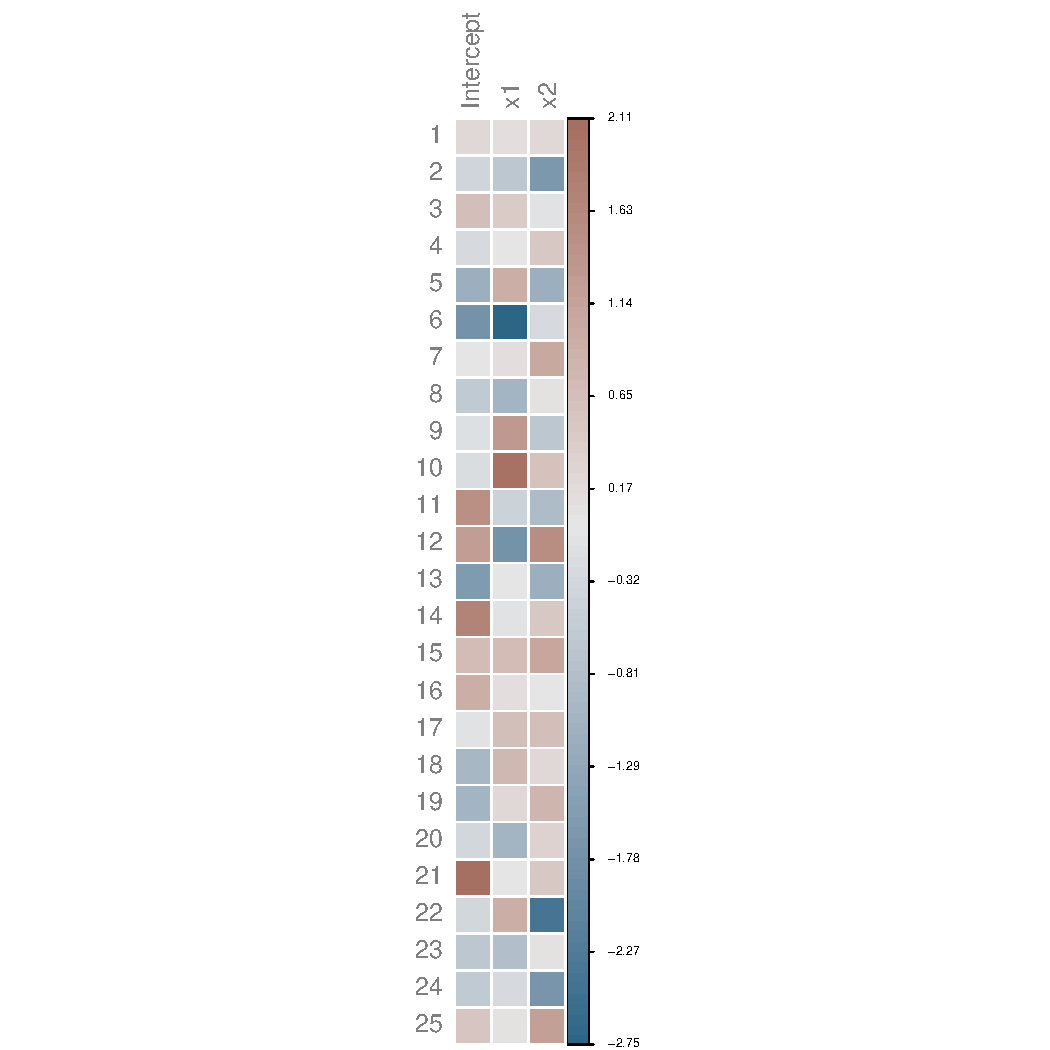
\includegraphics[scale=.35, center]{coefCorrplot}}

Let's say as a precursor to a mixed model, you want to run separate regressions on the levels of the grouping factor within which observations are nested.  Furthermore, you want to make a graph that reflects the coefficients values, fading them out and make them smaller as they tend toward zero.  First think about the steps you'd have to take in your own package, then note that this technically can be a one line operation in R\sidenote{For visualization purposes only, I scale the matrix of coefficients so that they can be on equal visual footing. The purpose here would never be for inference.}. The plot is shown to the right with additional options specified, and further down to it I show a similar plot, which looks at model for two dependent variables and 46 countries.

\marginnote{\includegraphics[scale=.30, center]{"Color as Tile"}}
\begin{knitrout}\footnotesize
\definecolor{shadecolor}{rgb}{0.969, 0.969, 0.969}\color{fgcolor}\begin{kframe}
\begin{alltt}
\hlkwd{library}\hlstd{(lme4);} \hlkwd{library}\hlstd{(corrplot)}
\hlkwd{corrplot}\hlstd{(}\hlkwd{scale}\hlstd{(}\hlkwd{coef}\hlstd{(}\hlkwd{lmList}\hlstd{(y} \hlopt{~} \hlstd{x1} \hlopt{+} \hlstd{x2} \hlopt{|} \hlstd{g, mydata))),} \hlkwc{is.corr}\hlstd{=F)}
\end{alltt}
\end{kframe}
\end{knitrout}

It's assumed if folks could do this sort of thing easily in other statistical packages they would be doing so.  R users by contrast are doing things like this all the time as standard practice, and R allows them to take their models further much more easily. Now let's look at some other advanced models.

\begin{knitrout}\footnotesize
\definecolor{shadecolor}{rgb}{0.969, 0.969, 0.969}\color{fgcolor}\begin{kframe}
\begin{alltt}
\hlcom{# multiple regressions, same predictors}
\hlkwd{lm}\hlstd{(}\hlkwd{cbind}\hlstd{(y1, y2, y3)} \hlopt{~} \hlstd{x1} \hlopt{+} \hlstd{x2)}

\hlcom{# generalized additive model (mgcv package)}
\hlkwd{gam}\hlstd{(y} \hlopt{~} \hlkwd{s}\hlstd{(x1)} \hlopt{+} \hlkwd{s}\hlstd{(x2))}

\hlcom{# mixtures of regessions (flexmix package)}
\hlkwd{flexmix}\hlstd{(y} \hlopt{~} \hlstd{x1} \hlopt{+} \hlstd{x2,} \hlkwc{k}\hlstd{=}\hlnum{3}\hlstd{)}

\hlcom{# bayesian regression (bayesglm package)}
\hlkwd{bayesglm}\hlstd{(y} \hlopt{~} \hlstd{x1} \hlopt{+} \hlstd{x2,} \hlkwc{family}\hlstd{=}\hlstr{'poisson'}\hlstd{)}

\hlcom{# optimization with likelihood function}
\hlstd{lmLL} \hlkwb{=} \hlkwa{function}\hlstd{(}\hlkwc{par}\hlstd{)\{}
  \hlstd{beta} \hlkwb{=} \hlstd{par[}\hlopt{-}\hlnum{1}\hlstd{]}
  \hlstd{sigma} \hlkwb{=} \hlstd{par[}\hlnum{1}\hlstd{]}
  \hlstd{mu} \hlkwb{=} \hlstd{X}\hlopt\hlstd{beta}
  \hlopt{-}\hlkwd{sum}\hlstd{(}\hlkwd{dnorm}\hlstd{(y, mu, sigma,} \hlkwc{log}\hlstd{=T))}
\hlstd{\}}
\hlkwd{optim}\hlstd{(}\hlkwc{par}\hlstd{=startingvalues,} \hlkwc{fun}\hlstd{=lmLL)}

\hlcom{# classical time series}
\hlkwd{arima}\hlstd{(y,} \hlkwc{order}\hlstd{=}\hlkwd{c}\hlstd{(}\hlnum{0}\hlstd{,} \hlnum{1}\hlstd{,} \hlnum{1}\hlstd{))}
\end{alltt}
\end{kframe}
\end{knitrout}

You get the picture.  Modeling is as easy in R as it would be in other packages, if not easier in many cases. In addition, you get access to more models and more flavors of the models\sidenote{As an example, the \texttt{\textcolor{red}{ols}} in the \emph{\textcolor{blue}{Hmisc}} package would do even more for your standard regression (and logistic,s survival and other) models.}, not to mention various approaches that are at the cutting edge of statistical science.  Furthermore, you can simply do more with your model results once you have them.  Users of other statistical packages are stuck with  older approaches, commands that won't work if you try to use them in any nonstandard fashion, and modeling functions for which one has no way to see what the commands are actually doing.  


% !Rnw root = DDR.Rnw



\part{Visualization}

I'm not going to talk a lot about visualization in R, it's been ahead of other statistics packages in that department at least since version 1.0\sidenote{Look at \href{http://www.r-project.org/}{R's homepage}, this plot is over 10 years old, and would still be impossible for most statistics packages (code available if you click on the image at the website).
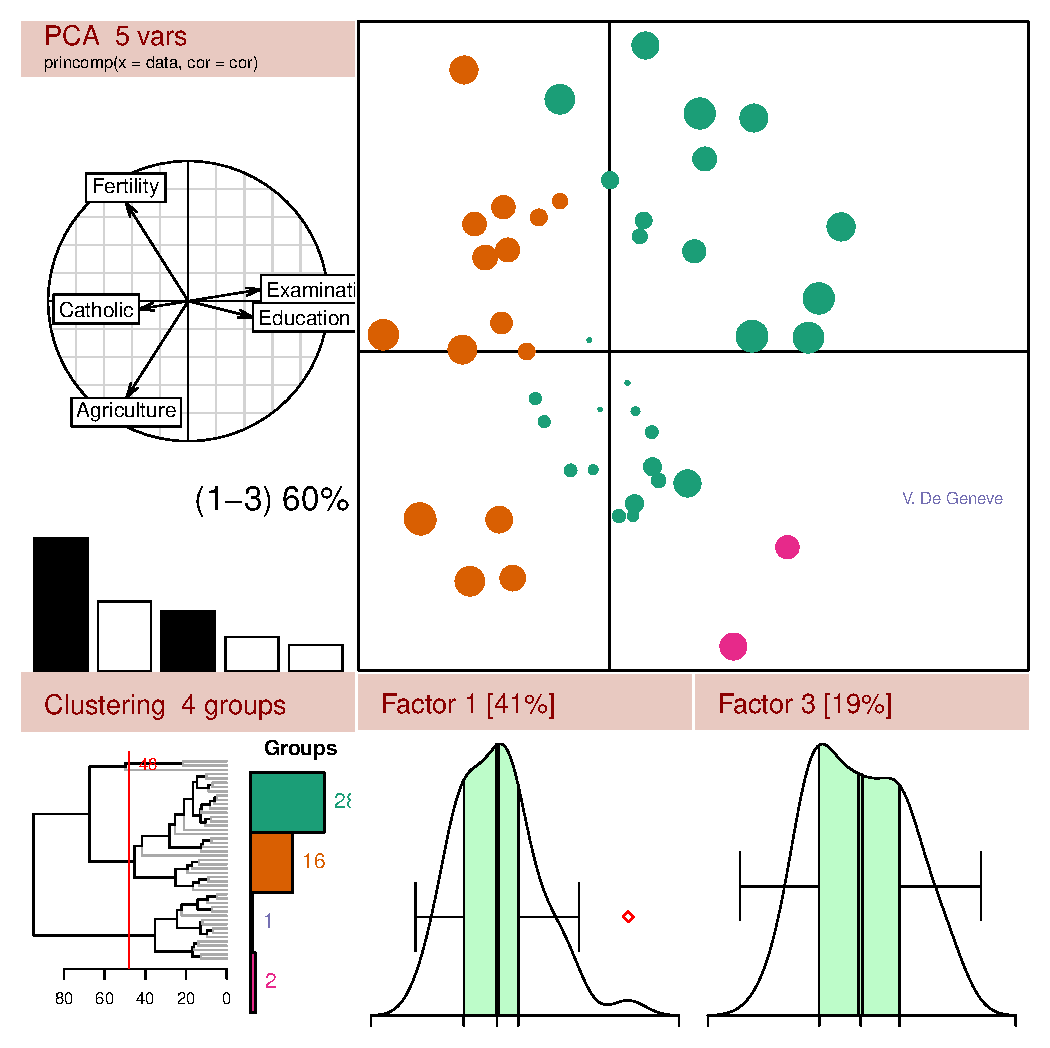
\includegraphics[scale=.25]{rhome}}. Admittedly traditional statistics packages have finally started to make gains in this area in recent years, but even as they do R continues to move the goalposts.

I will show how easy it is to get standard plots, but it's more or less a waste of R's capabilities if this is all you want to use it for.

\begin{knitrout}\footnotesize
\definecolor{shadecolor}{rgb}{0.969, 0.969, 0.969}\color{fgcolor}\begin{kframe}
\begin{alltt}
\hlkwd{barplot}\hlstd{(}\hlkwd{table}\hlstd{(d))}
\hlkwd{plot}\hlstd{(x, y)}
\hlkwd{stripchart}\hlstd{(x} \hlopt{~} \hlstd{g,} \hlkwc{col}\hlstd{=}\hlkwd{rainbow}\hlstd{(}\hlnum{10}\hlstd{),} \hlkwc{pch}\hlstd{=}\hlnum{20}\hlstd{)}
\hlkwd{hist}\hlstd{(x)}
\end{alltt}
\end{kframe}
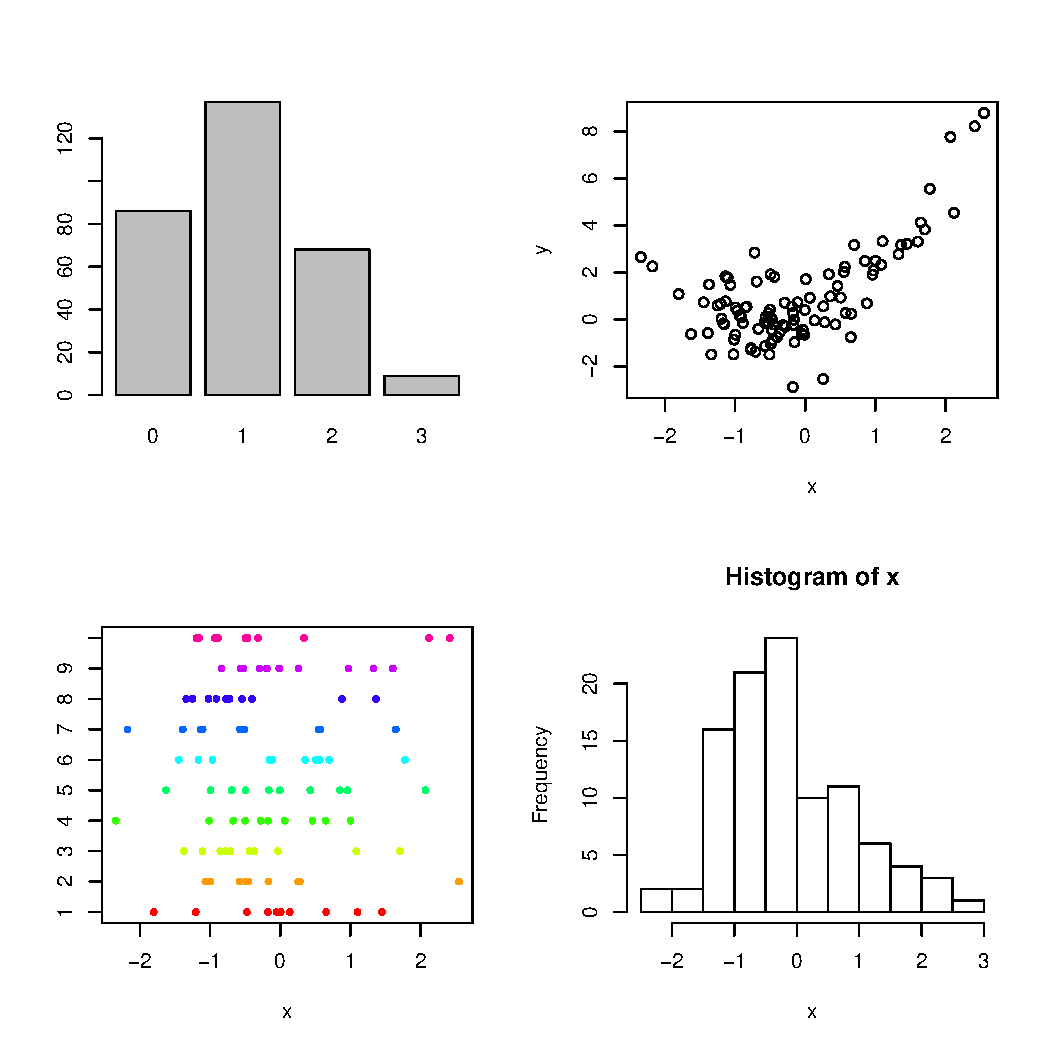
\includegraphics[width=\maxwidth]{figure/basicvis} 

\end{knitrout}

For one, these convey too little information.  You don't need a visualization for something you can describe in a short sentence. \emph{But even if this is all you're doing visually}, you'd still be better off in R because you would have fine control over every aspect of the plot and be able to tweak anything about it that you'd want to.  

But let's stick with standard plots and show how easy it is to get something better. As an example I'll show a scatterplot using the car package.

\begin{knitrout}\footnotesize
\definecolor{shadecolor}{rgb}{0.969, 0.969, 0.969}\color{fgcolor}\begin{kframe}
\begin{alltt}
\hlkwd{library}\hlstd{(car)}
\hlkwd{scatterplot}\hlstd{(x, y,} \hlkwc{ellipse}\hlstd{=T)}
\end{alltt}
\end{kframe}

{\centering 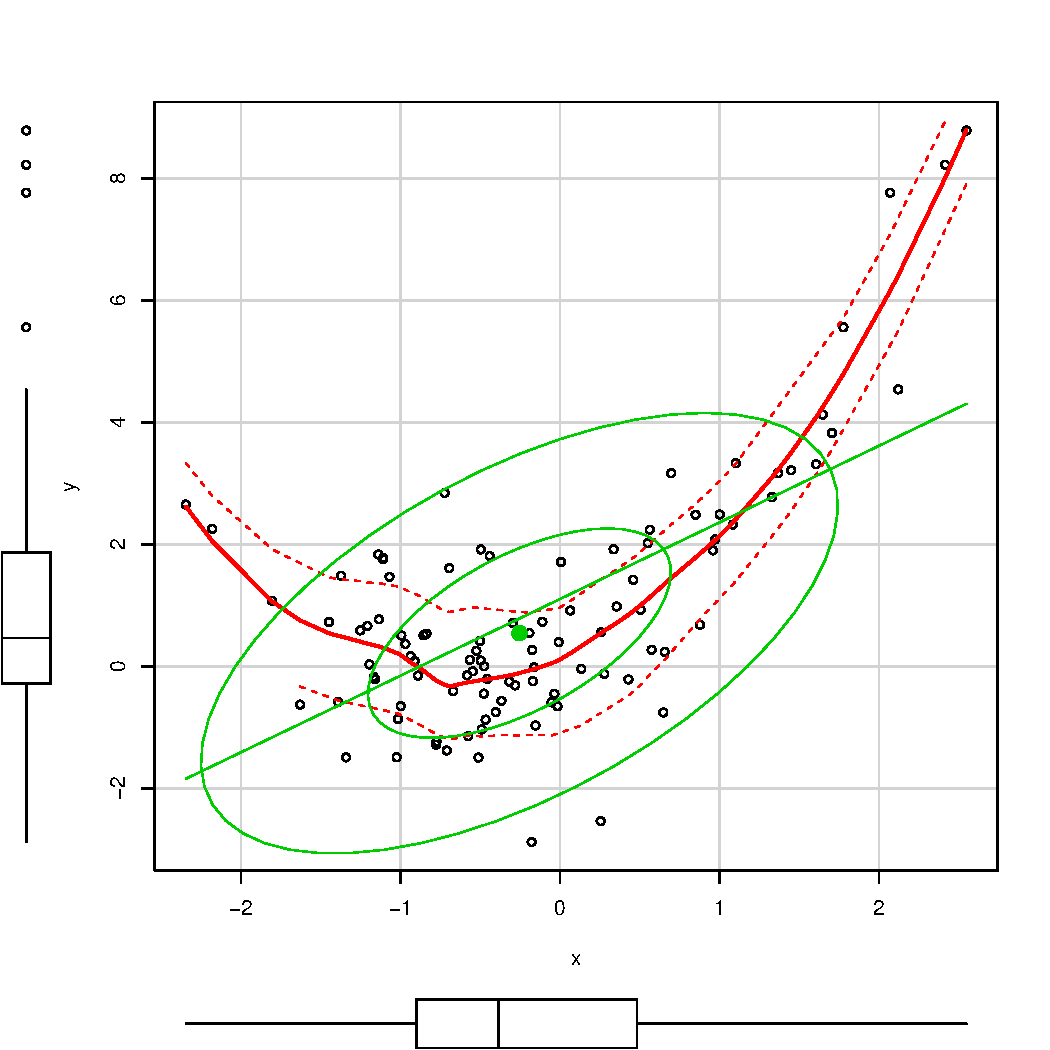
\includegraphics[width=.49\linewidth]{figure/carDemo} 

}



\end{knitrout}

With no additional coding effort you have an enhanced scatterplot, a smooth and linear function imposed on it, a data concentration ellipse based on a bivariate normal distribution, univariate boxplots in the margins, and the ability to identify points of interest interactively.  It actually would take little effort to reproduce most of the scatterplot with the ggplot2 package or even the base R plotting capabilities.

\begin{knitrout}\footnotesize
\definecolor{shadecolor}{rgb}{0.969, 0.969, 0.969}\color{fgcolor}\begin{kframe}
\begin{alltt}
\hlkwd{library}\hlstd{(ggplot2)}
\hlkwd{ggplot}\hlstd{(}\hlkwd{aes}\hlstd{(x, y),} \hlkwc{data}\hlstd{=gd)} \hlopt{+}
  \hlkwd{geom_point}\hlstd{()} \hlopt{+}
  \hlkwd{geom_smooth}\hlstd{(}\hlkwc{col}\hlstd{=}\hlstr{'red'}\hlstd{,} \hlkwc{se}\hlstd{=T)} \hlopt{+}
  \hlkwd{geom_smooth}\hlstd{(}\hlkwc{col}\hlstd{=}\hlstr{'lightgreen'}\hlstd{,} \hlkwc{method}\hlstd{=}\hlstr{'lm'}\hlstd{,} \hlkwc{se}\hlstd{=F)} \hlopt{+}
  \hlkwd{theme_minimal}\hlstd{()}

\hlkwd{plot}\hlstd{(x, y,} \hlkwc{pch}\hlstd{=}\hlnum{19}\hlstd{)}
\hlkwd{abline}\hlstd{(}\hlkwd{lm}\hlstd{(y}\hlopt{~}\hlstd{x),} \hlkwc{col}\hlstd{=}\hlstr{'lightgreen'}\hlstd{)}
\hlkwd{lines}\hlstd{(}\hlkwd{data.frame}\hlstd{(x,} \hlkwd{predict}\hlstd{(}\hlkwd{loess}\hlstd{(y}\hlopt{~}\hlstd{x)))[}\hlkwd{order}\hlstd{(x),],} \hlkwc{col}\hlstd{=}\hlstr{'red'}\hlstd{)}
\end{alltt}
\end{kframe}
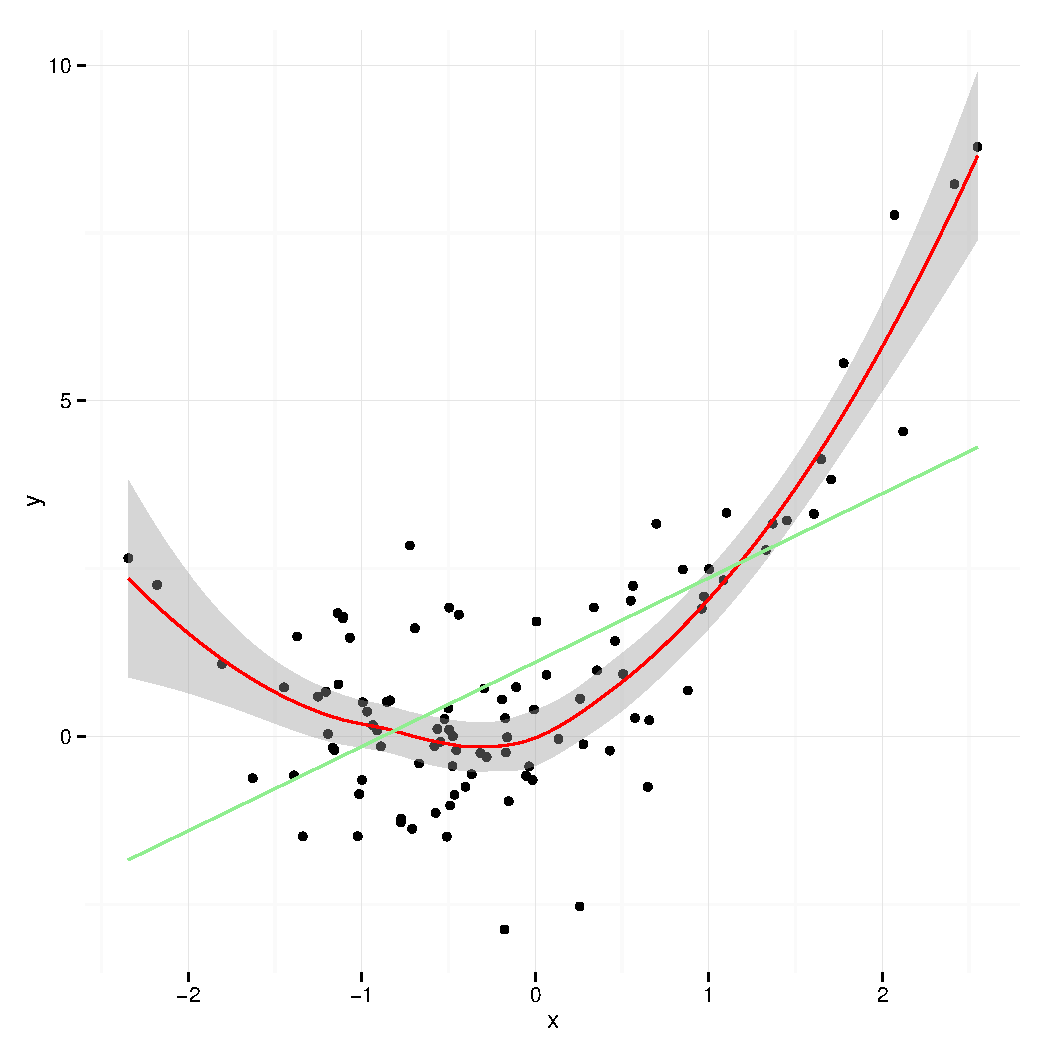
\includegraphics[width=.49\linewidth]{figure/ggCarScatter1} 
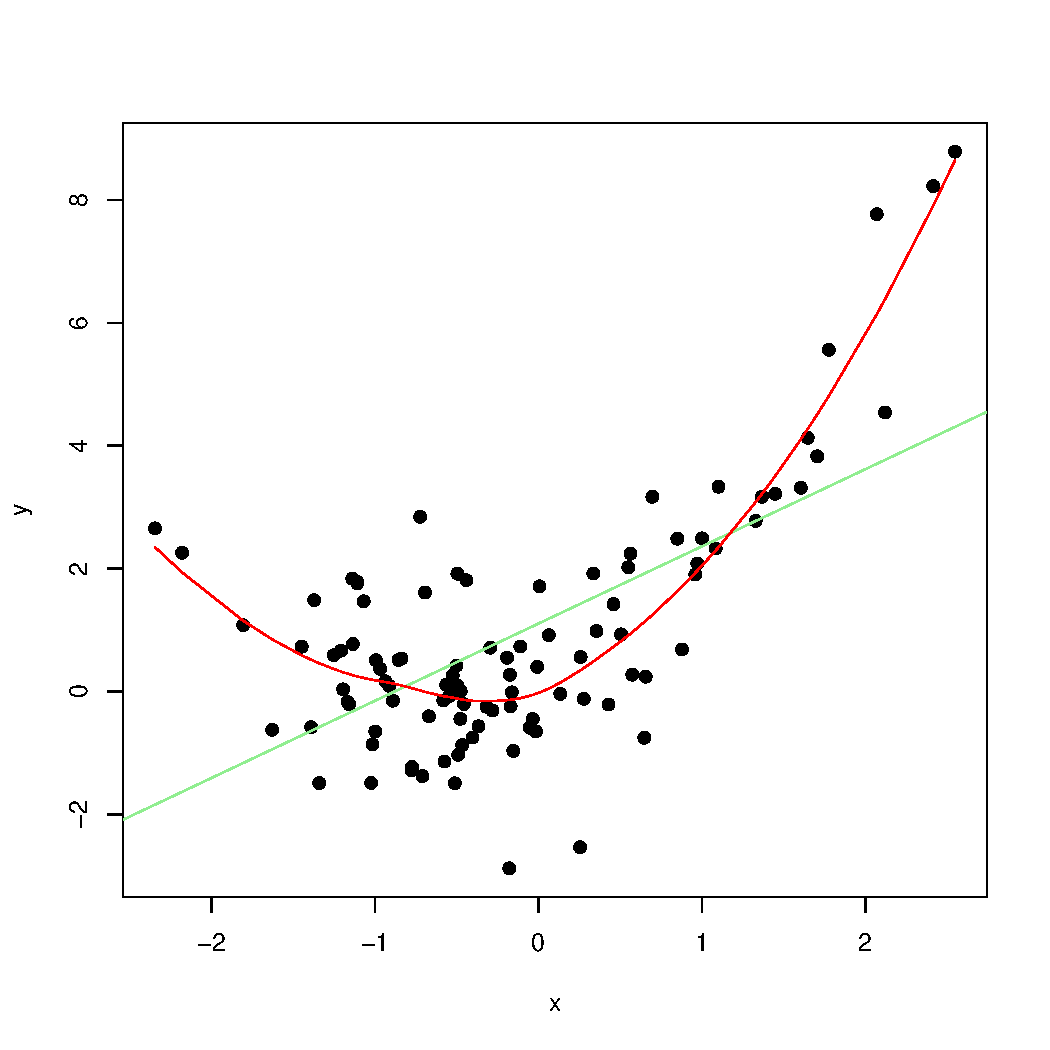
\includegraphics[width=.49\linewidth]{figure/ggCarScatter2} 

\end{knitrout}


\noindent Maybe you want a 3d scatterplot with a with smooths for different groups?  Again this is one line of code.

\begin{knitrout}\footnotesize
\definecolor{shadecolor}{rgb}{0.969, 0.969, 0.969}\color{fgcolor}\begin{kframe}
\begin{alltt}
\hlkwd{scatter3d}\hlstd{(y} \hlopt{~} \hlstd{x1} \hlopt{+} \hlstd{x2} \hlopt{|} \hlstd{x0,} \hlkwc{data}\hlstd{=d,} \hlkwc{fit}\hlstd{=}\hlstr{'additive'}\hlstd{)}
\end{alltt}
\end{kframe}
\end{knitrout}
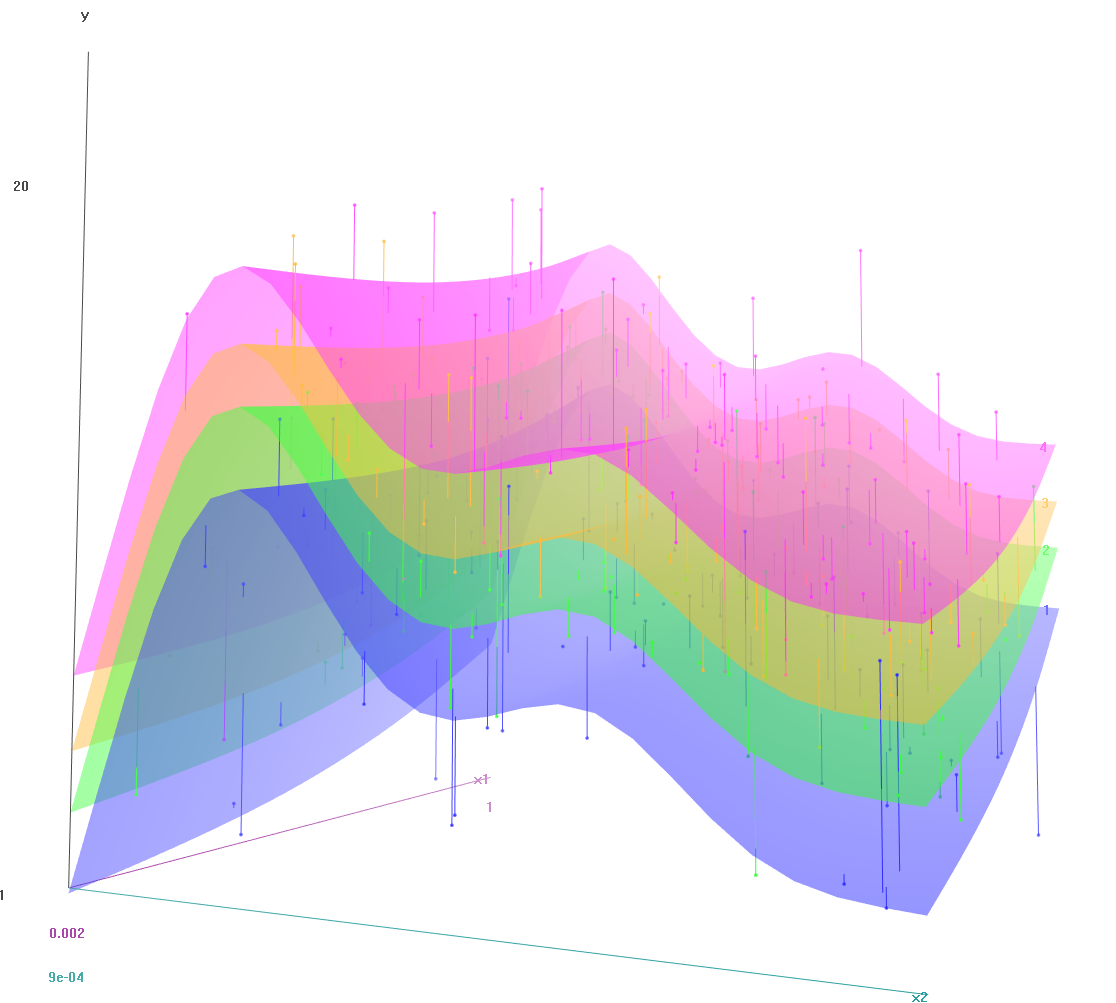
\includegraphics[scale=.25]{gam3d}

I provide the above examples not to show that R can do this or that visualization while statistical packages can't.  The point is not that other statistical packages can't do the same kinds of visualizations you want, although that is sometimes, if not often, going to be the case.  It's just going to typically be easier, often much easier, in R to get far better versions of standard plots, so that you'll be spending most of your time tweaking the visualization you actually wanted to get it just the way you want it, rather than fighting with a program that hasn't put much relative effort into visualization and in the end eventually settling on whatever it gives you.


For a comparison I looked up "'statistics package' visualization" and the results are as follows.  SAS, has an \href{http://www.sas.com/en_us/insights/big-data/data-visualization.html}{unnecessarily shaded bar plot} as the first thing it shows regarding its visualization module.  SPSS as usual wants you to pay for this capability, and its \href{http://www-03.ibm.com/software/products/en/spss-viz-designer}{screenshots} suggest it's way too much.  I couldn't find much on the topic with Stata that actually showed much beyond the standard graphics, and in any case it has never been known for its prowess there.  Honestly, you'd be better of using other visualization-specific tools freely available on the web even if you were wed to SAS, SPSS, Stata etc.  But as a comparison, here are the sorts of things R visualization entails- \href{http://shiny.rstudio.com/gallery/}{shiny}, \href{http://ggvis.rstudio.com/interactivity.html}{ggvis}.  Modern visualization must be interactive and web ready to go along with producing high quality static graphics, and R has tools ready for you to go there.





% !Rnw root = DDR.Rnw



\part{Programming in R}
Something that would surprise those coming from traditional statistics packages is the fact that it is actually much easier to code in R.  It's already the case that data slicing, dicing, wrangling, cleaning etc. is easier in R because of the flexibility it gets from being a true, object-oriented programming language.  However even the act of coding itself is made easier with RStudio, the integrated development environment for R.  I'll list some features and you can ask yourself if you'd rather program in RStudio or the syntax editor of your statistical package.

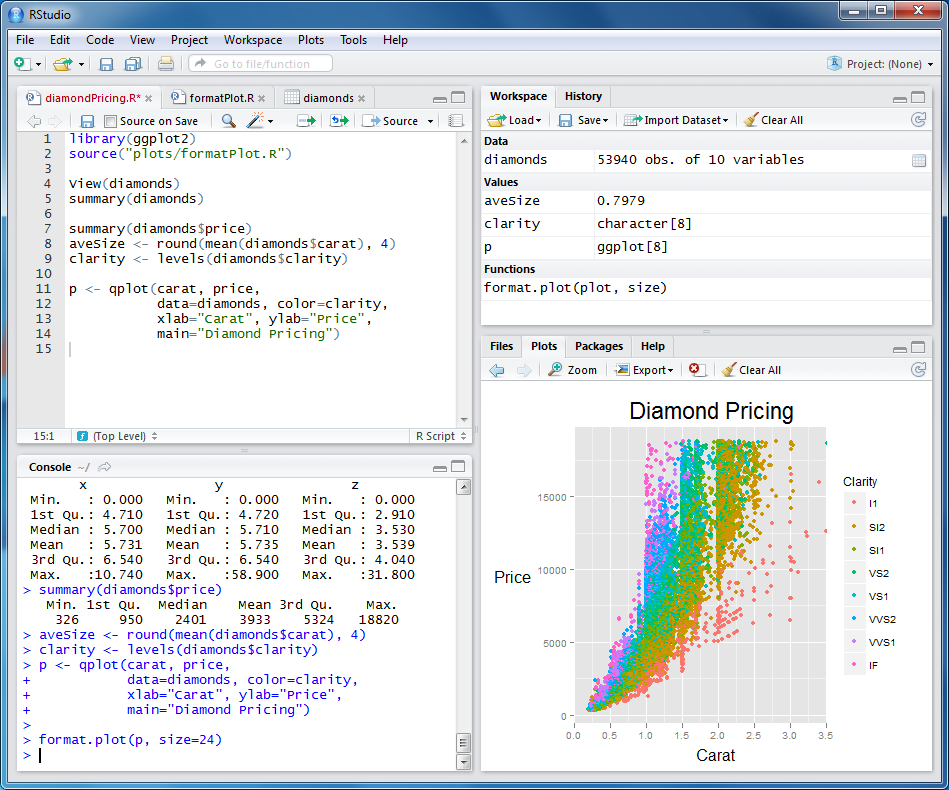
\includegraphics[scale=.25]{rstudio}

RStudio

\section{Basic Benefits}
With RStudio you get various base functions, strings, logicals and so forth highlighted as is common with many syntax editors, which makes reading code notably easier. In addition, RStudio has a searchable history, auto-completes object names, closes all manner of brackets, and closes quotation marks, auto-indents etc. making it far less likely to have, e.g. a left off parenthesis, to break your code.  The auto-indent helps keep loops and so forth tidy and more legible automatically. And finally, it's nice to know you'll never lose anything, as RStudio auto-saves every few seconds.  You can open 10 scripts, not save any of them, close RStudio, open it back up, and it'd all be just as you left it.  Many other core features can be found at \href{http://www.rstudio.com/products/rstudio/features/}{RStudio's website}.


\section{Code Maneuverability} Let's say you are staring at 100 lines of code on one of several R scripts you are working on, and your cursor is currently at line 50 and you want to do the following steps: run everything to that line, pop to the console for a quick one-off graph, go back to where you were in the script, open the help file for the function you're currently using, look at the source code for it, run the rest of the code from that line on, switch to the script 3 tabs down, switch back, rerun, what you the last bit of code you ran, switch to the next tab (which is a markdown script), check the spelling and compile the script to pdf or html.  To do this in RStudio would take about 20 keystrokes and no mouse movement at all\sidenote{You can see all the shortcuts in RStudio \href{https://support.rstudio.com/hc/en-us/articles/200711853-Keyboard-Shortcuts}{here}}.  This is actually a common sort of capability in IDEs, and you'll find similar functionality in others that are geared toward other programming languages (just not statistical packages).  And for those that don't care much for programming, they should want to spend less time doing it, but my guess is that the easier it is for someone to program the more likely they will start to enjoy it.


\section{Project Management}
RStudio allows one to create projects, which are like self-contained collections of scripts housed in their own directory. Say you're a faculty member and you're working on a book, and have two current research projects.  You could be writing the book in one project that has, for example, separate scripts for each chapter. In another are the analysis scripts pertaining to that research, and the same for your other research endeavor.   You're working on your book when a colleague calls up and asks you to rerun part of an analysis for her.  You simply switch to that project, and RStudio brings up all the scripts you had when you were working on it.  When done you just go back to the book project and it will be as though you never left\sidenote{I'll point out you wouldn't even need the mouse to do this.}.  Furthermore, these projects are capable of being tied to Git or Subversion for version control, making it more easy to collaborate on these projects with colleagues.  You can also have RStudio settings specific to each project, and have package management specific to each project.


\section{Support for Literate Programming \& Reproducible Research}
The time has come for researchers to get more serious about their data, how they produce the results of their research, and conducting analysis in a fashion that is reproducible.  Research results in publication form are almost entirely thought of as a finished product among social scientists, but those days are over.  Better work results from assuming the final product will be dynamic, easily updated, and make it as easy as possible to reproduce the results.One never has to leave the R environment to go from data to journal ready publication, while engaging in best practices for reproducible research. R has long been in this game, as tools like Sweave have been around since the days of S\marginnote{I found it telling that searching for "reproducible research" and "SPSS" has a first link at IBM to calling R from SPSS.}. 

\subsection{Document Production}
RStudio makes it easy to use R to take your code and analysis and produce high-quality, publish-ready documents, and in a variety of ways.  As mentioned, RStudio takes \LaTeX and with various R tools like the \emph{\textcolor{blue}{knitr}} package, and compiles the text, code and results into a final pdf.  If I were producing a an article based on statistical results, it would be trivial to update the models and thus update results.  The following code uses the \emph{\textcolor{blue}{stargazer}} package write model results out to a file in \LaTeX, using the style of the American Journal of Political Science, which can then be imported directly into the document file.

\begin{knitrout}\footnotesize
\definecolor{shadecolor}{rgb}{0.969, 0.969, 0.969}\color{fgcolor}\begin{kframe}
\begin{alltt}
\hlstd{mod} \hlkwb{=} \hlkwd{lm}\hlstd{(y} \hlopt{~} \hlstd{x1} \hlopt{+} \hlstd{x2)}
\hlstd{stargazer::}\hlkwd{stargazer}\hlstd{(mod,} \hlkwc{out}\hlstd{=}\hlstr{'metaLaTeX.Rnw'}\hlstd{,} \hlkwc{style}\hlstd{=}\hlstr{'ajps'}\hlstd{)}
\end{alltt}
\end{kframe}
\end{knitrout}

\input{metaLaTeX.Rnw}


In this way we can always update the document based on new data, discovered bugs, or maybe try enhanced analysis.  The document doesn't have to stay frozen in time with all its possible foibles.  This is something that wasn't possible when print outlets were the primary way to dispense scientific information.  Now the web and digital presentation are not only desired they are assumed.  Now we can think of research articles having version numbers just like software, with relevant updates and enhanced 'features'.

\subsection{Web-based Presentation}
It might actually be even easier with RStudio to produce a web-ready document.  R has its own flavor of \href{http://daringfireball.net/projects/markdown/}{Markdown}, text-to-HTML conversion tool widely used to produce content for the web.


\begin{footnotesize}
\begin{verbatim}
---
title: "MyTitle"
author: "Me"
date: "Monday, August 11, 2014"
output: html_document
---

This is an R Markdown document. Markdown is a simple formatting syntax for authoring 
HTML, PDF, and MS Word documents. For more details on using R Markdown 
see <http://rmarkdown.rstudio.com>.

When you click the **Knit** button a document will be generated that includes both 
content as well as the output of any embedded R code chunks within the document. 
You can embed an R code chunk like this:

```{r}
summary(cars)
```

You can also embed plots, for example:

```{r, echo=FALSE}
plot(cars)
```

Note that the `echo = FALSE` parameter was added to the code chunk to prevent 
printing of the R code that generated the plot.
\end{verbatim}
\end{footnotesize}

\bigskip
\noindent That code will produce the following webpage.
\bigskip

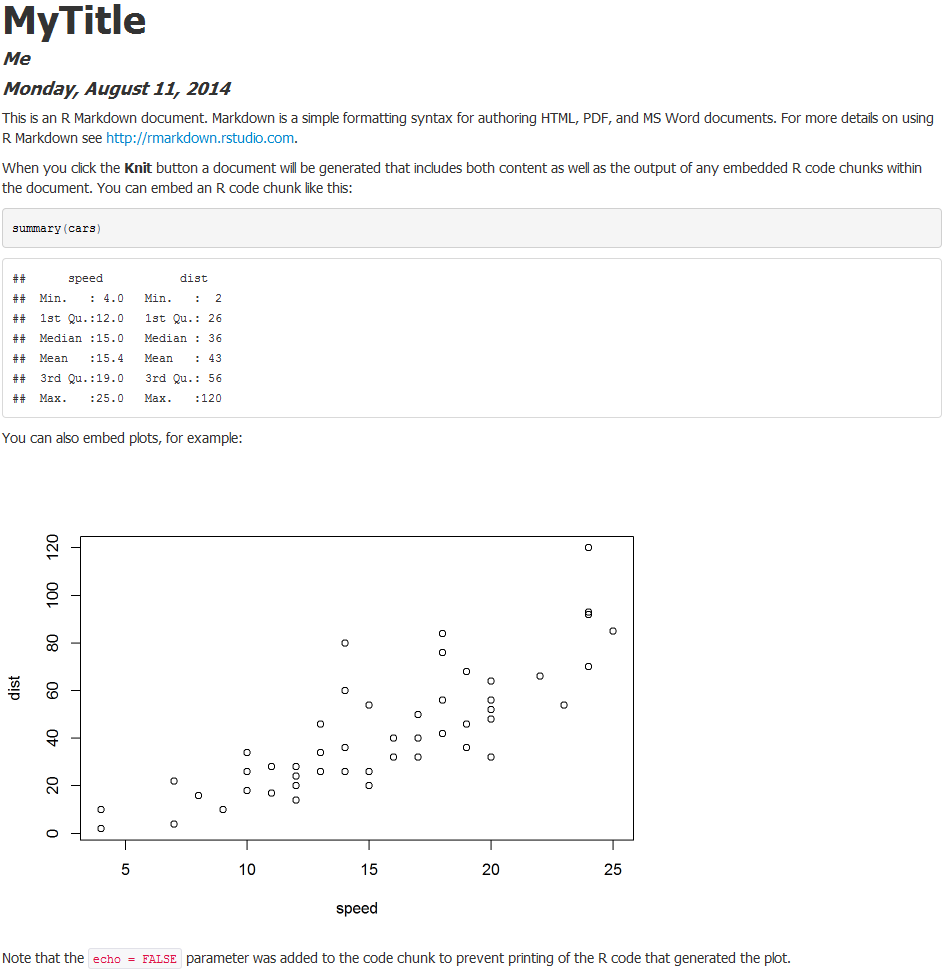
\includegraphics[scale=.25]{rmarkdown}

In addition, R can make html5 presentations.  I have an example \href{http://www3.nd.edu/~mclark19/learn/presentation/RI/#1}{here} that I use for my R short course.  So now you can do you research presentations with code and results included as well, and again you've never had to leave the RStudio.  I guess I should mention you can use markdown for MS Word documents, but I haven't yet figured out why one would want to.

\subsection{Version Control}
Along with all of this, RStudio projects incorporate \href{https://support.rstudio.com/hc/en-us/articles/200532077-Version-Control-with-Git-and-SVN}{version control}, enabling collaborative research where you don't have to worry about the data, and can easily keep track of changes to data and code, revert if necessary etc.  If you're wondering why you'd need version control, I'll let the following list from \href{http://stackoverflow.com/questions/1408450/why-should-i-use-version-control}{stackoverflow}.


\begin{quote}
Have you ever:
\begin{itemize}
  \item Made a change to code, realized it was a mistake and wanted to revert back?
  \item Lost code or had a backup that was too old?
  \item Had to maintain multiple versions of a product?
  \item Wanted to see the difference between two (or more) versions of your code?
  \item Wanted to prove that a particular change broke or fixed a piece of code?
  \item Wanted to review the history of some code?
  \item Wanted to submit a change to someone else's code?
  \item Wanted to share your code, or let other people work on your code?
  \item Wanted to see how much work is being done, and where, when and by whom?
  \item Wanted to experiment with a new feature without interfering with working code?
\end{itemize}

In these cases, and no doubt others, a version control system should make your life easier. 
\end{quote}

I'll add that most of those apply to both data and documents as well, and version control works for those just like it does for code.  It's indispensable for collaborations.  You and co-authors can work on documents, data, and analysis without worry, and always know what you're working with.


\section{Functions \& Debugging}
R makes even makes it easy to write your own functions, which can make many operations easier and contributes to reproducibility as well.  But you don't have be an advanced R programmer.  You could simply change the defaults for some function you like to use, for example.  However, in the following we'll demonstrate writing an original function, one that takes 3 inputs (arbitrarily named 'a' 'b' and 'c'), and takes the sum of the first two and multiplies it by the third input.

\begin{knitrout}\footnotesize
\definecolor{shadecolor}{rgb}{0.969, 0.969, 0.969}\color{fgcolor}\begin{kframe}
\begin{alltt}
\hlstd{myfunc} \hlkwb{=} \hlkwa{function}\hlstd{(}\hlkwc{a}\hlstd{,} \hlkwc{b}\hlstd{,} \hlkwc{c}\hlstd{)\{}
  \hlstd{result} \hlkwb{=} \hlstd{(a} \hlopt{+} \hlstd{b)} \hlopt{*} \hlstd{c}
  \hlstd{result}
\hlstd{\}}

\hlkwd{myfunc}\hlstd{(}\hlnum{1}\hlstd{,} \hlnum{2}\hlstd{,} \hlnum{3}\hlstd{)}
\end{alltt}
\begin{verbatim}
## [1] 9
\end{verbatim}
\end{kframe}
\end{knitrout}

Many R functions are quite complex, but yours just has to do what you need to.  You can also do so within other functions implicitly if it's very simple.  The following uses the \texttt{\textcolor{red}{sapply}}, which applies some function to all elements of a vector or list, and in this case we'll make that same calculation to the list elements\sidenote{Some of you may be wondering where the loop is.  In R, it is typically easier, and often clearer, to not use explicit loops.}.

\begin{knitrout}\footnotesize
\definecolor{shadecolor}{rgb}{0.969, 0.969, 0.969}\color{fgcolor}\begin{kframe}
\begin{alltt}
\hlstd{mylist} \hlkwb{=} \hlkwd{list}\hlstd{(}\hlkwd{c}\hlstd{(}\hlnum{1}\hlstd{,}\hlnum{2}\hlstd{,}\hlnum{3}\hlstd{),} \hlkwd{c}\hlstd{(}\hlnum{3}\hlstd{,}\hlnum{2}\hlstd{,}\hlnum{1}\hlstd{),} \hlkwd{c}\hlstd{(}\hlnum{1}\hlstd{,}\hlnum{1}\hlstd{,}\hlnum{1}\hlstd{))}

\hlkwd{sapply}\hlstd{(mylist,} \hlkwa{function}\hlstd{(}\hlkwc{listelem}\hlstd{) (listelem[}\hlnum{1}\hlstd{]} \hlopt{+} \hlstd{listelem[}\hlnum{2}\hlstd{])} \hlopt{*} \hlstd{listelem[}\hlnum{3}\hlstd{])}
\end{alltt}
\begin{verbatim}
## [1] 9 5 2
\end{verbatim}
\end{kframe}
\end{knitrout}


In this case the implicit function takes a an element from the list (now arbitrarily named listelem), each of which contains three values, and does the same operation as before.  \marginnote{My own rule of thumb is that if I'm using a chunk of similar code more than twice, it's time to write a function that does what the code does.} Unlike other statistical packages where you practically have to be an expert to create and program your own commands to use, or it's simply an otherwise discouraging process, it's pretty easy to do in R, and you'll save a lot of programming time the more you do it.

Furthermore, R and RStudio have a debugging system that makes it easy to spot problems, find time bottlenecks, cycle through all iterations of loops etc.  So for those that get more involved with coding or want to write a complex function, it will likely be a lot easier to do in R.





%%%%%%%%%%%%%%%%%%%%%%%%%%%%%%%%%%%%%%
\part{Summary}
Before wrapping things up, let's talk about some of the other things R can do.  These are just some of things that should/would be of interest to any applied social scientist, but are not the sorts of things typically covered in a social science stats course, nor are they easily done or common in statistics packages they normally use.  With R you have a lot of functionality for things like web scraping, machine learning, text analysis, Bayesian estimation, mapping and geospatial modeling, direct access to data repositories, accessing social media streams, the ability to interface with newspaper and journal APIs, and a whole host of tools from other sciences that might be of use for their particular research.  R's audience is very general, and its users build tools to meet their needs and make them available for others.  You will typically have a lot of choice in how you do any particular thing in R modeling or otherwise, unlike other packages for which you may have only one or two commands that don't provide much different content.  It may be overwhelming at first introduction, but it is very freeing.  You'll soon that the question isn't 'Can R do this?', it's 'What package in R does this?'.


Hopefully this document will give the SAS, SPSS, Stata etc. users in social science some things to think about.  Those are fine programs in their own right, but unless you are a great programmer with their syntax, using them is less efficient than what you can do with only a basic knowledge of R.  A lot of folks think there is a steep learning curve just to get into R, but for purely applied use of just importing data and running a model, it can be used in pretty much the same way as one does the other statistical packages, so you can pop over to it to do the things your own package doesn't do the way you would like.  But even with purely applied use, there are efficiency gains due to its object-oriented programming features, RData files, R Projects, visualization etc., and the more you get used to it the more you'll get out of your data.  

Modern science is dynamic, interactive, web-based, and reproducible.  R has all the tools you need for modern scientific research in any discipline.  Spend some time at \href{http://www.r-bloggers.com/}{R-bloggers} to see what people are doing with R.  It will make your head spin.  But know that many of them aren't expert programmers or statisticians either, and if they can use R to do those things, you can too.  




\end{document}
